\documentclass[isoft]{ssltexposter}

\usepackage{lipsum}
\usepackage{natbib}
\usepackage{booktabs}
%\usepackage{subfig} 
\usepackage{amsmath} 
\usepackage{textcomp} 
\usepackage{url}  
\usepackage[hidelinks]{hyperref}
\usepackage[utf8]{inputenc}
\usepackage[english]{babel}
%\usepackage{graphicx}
\usepackage{caption}
%\usepackage{subcaption}
%\usepackage[demo]{graphicx}
\usepackage{subfig}
\usepackage{tikz}
\usetikzlibrary{backgrounds, automata, positioning, arrows.meta, calc}
%No indent
\setlength\parindent{0pt}

%Space before and after some commands
\usepackage{titlesec}
%\titlespacing{\section}{0pt}{\parskip}{-\parskip}
%\titlespacing{command}{left spacing}{before spacing}{after spacing}[right]
\titlespacing{\section}{0pt}{1cm}{1cm}[\parskip]
%%%%%%%%%%%%%%%%%%%%%%%%%%%%%%%%%%%%%%%%%
%%               Configs               %%
%%%%%%%%%%%%%%%%%%%%%%%%%%%%%%%%%%%%%%%%%

%\newenvironment{localsize}[1]
%{%
%  %\clearpage
%  \let\orignewcommand\newcommand
%  \let\newcommand\renewcommand
%  \makeatletter
%  \input{bk#1.clo}%
%  \makeatother
%  \let\newcommand\orignewcommand
%}
%{%
%  \clearpage
%}

% Choose one of the section color {ufglhblue | ufgdkblue | dkblue | black | gold}
\setsectioncolor{blue!50!black}

% Define width of the rule or hide it by setting 0pt or commenting the command 
\setcolumnseprule{0pt}

% Inform the paths to the logo files or leave empty one or both parameters. 
% There are three options [ T | M | B ] to positioning them.
\setlogos[T]{images/[Logo] INFOTEC.png}

% Choose one of the background options {1 | 2 | 3}. 
% Actually, one can select any graphic file in backgrounds directory. 
%\setbackground{1c}

% Resize the title to keep it in two lines // {font size}{line height}
\settitlesize{64pt}{68pt}

% Resize the font of the content. Default {32pt}{38pt} // {font size}{line height}
\setcontentfontesize{26.5pt}{1pt}

% Resize the font of the emails. Default {26pt}{32pt} // {font size}{line height}
\setemailfontesize{2pt}{1pt}

% General info
\vspace{-1cm}\title{{\Large \uppercase{International Statistical Ecology Conference 2027}}\\
\hspace{5cm}\uppercase{\vspace{0.5cm}Modeling sowing timing under climate variability\\ using random walks on graphs}} 

\author{Isaac Vázquez Mendoza$^{1}$, Magali Arellano Vázquez$^{1}$.} 

% \department{Laboratório de Sinais e Sistemas\\Universidade Federal do ABC (UFABC)}

\email{%\fontsize{18pt}{1pt}\selectfont
$^1$INFOTEC Centro de Investigación e Innovación en Tecnologías de la Información y Comunicación.}

% \class{I Workshop do Laboratório de Sinais e Sistemas (WLSS)}

% \year{2019}


%Bottom line
\conference{}

%%%%%%%%%%%%%%%%%%%%%%%%%%%%%%%%%%%%%%%%%
%%           End configs               %%
%%%%%%%%%%%%%%%%%%%%%%%%%%%%%%%%%%%%%%%%%

\pagestyle{fancy}
\begin{document}
    \begin{poster}
    %%%%%%%%%%%%%%%%%%%%%%%%%%%%%%%%%%%%%%%%%
    %%             Begin poster            %%
    %%%%%%%%%%%%%%%%%%%%%%%%%%%%%%%%%%%%%%%%%
    
    %\begin{abstract}
    %    \normalsize
    %    
    %    \lipsum[57]
    %    
    %\end{abstract}
\section*{Introduction}




\section*{Section 1}


%\begin{center}
%\begin{figure}
%    \captionsetup{type=figure}
%    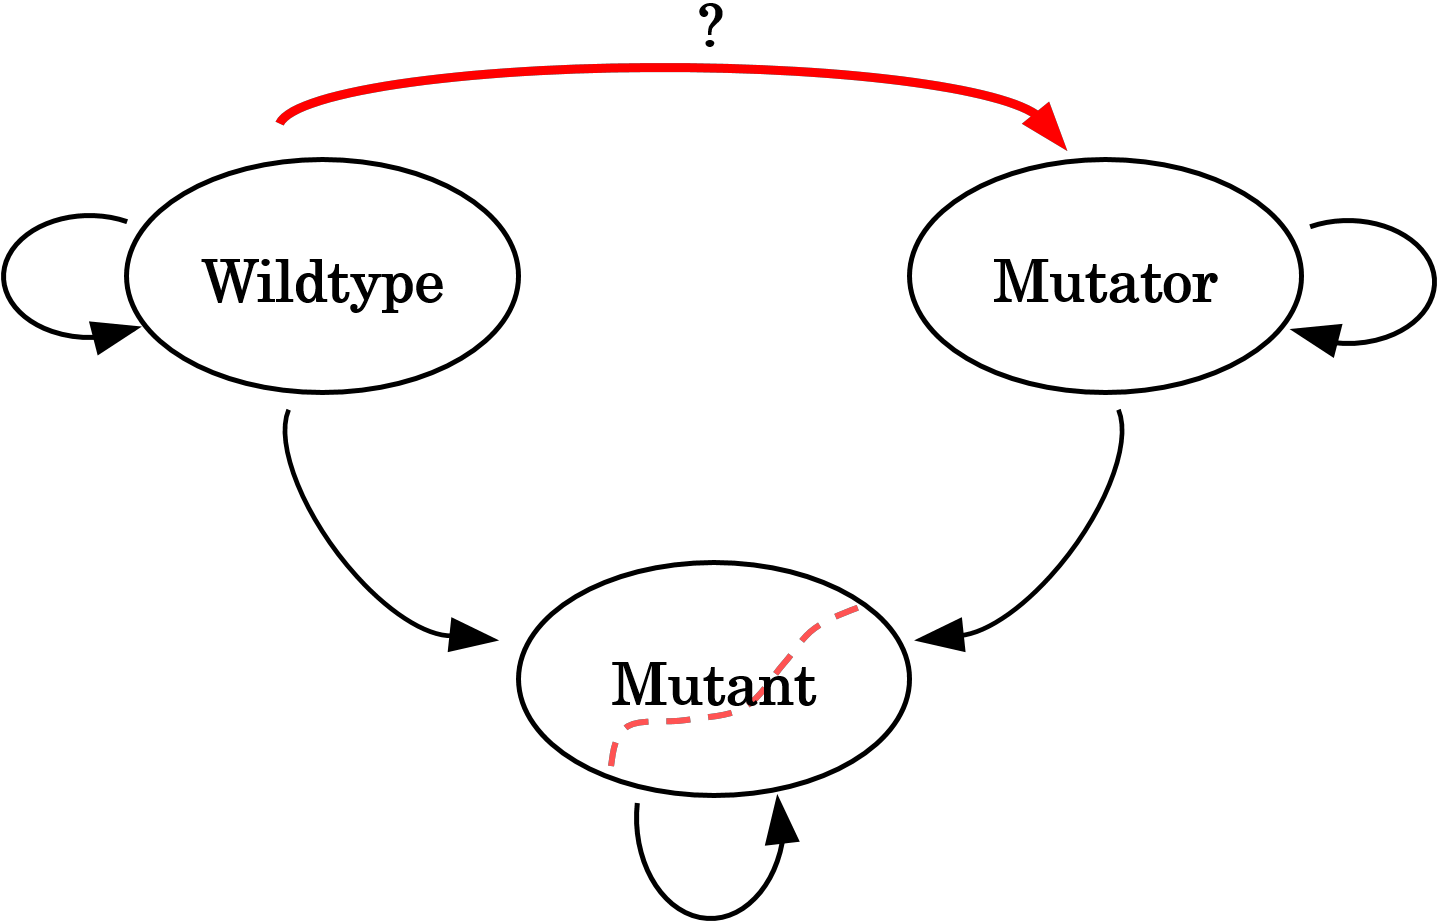
\includegraphics[scale=0.7]{images/Prop_mutante_cropped.png}
%    \caption{Dinámica de los fenotipos en células.}
%    \label{fig:fenotipo_mutador}               
%\end{figure}
%\end{center}




{
\centering

\resizebox{0.35\textwidth}{!}{%
    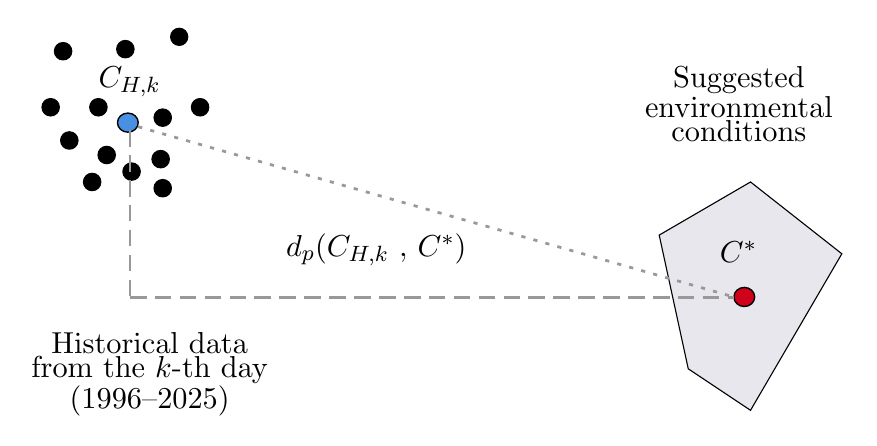
\begin{tikzpicture}[
        x=0.75pt,
        y=0.75pt,
        yscale=-1,
        xscale=1
    ]
			%uncomment if require: %\path (0,717); %set diagram left start at 0, and has height of 717
			
			%Shape: Axis 2D [id:dp4496072713140289] 
			%\draw  (58,700.13) -- (550,700.13)(64.03,422.4) -- (64.03,706.4) (540,695.13) -- (550,700.13) -- (540,705.13) (59.03,432.4) -- (64.03,422.4) -- (69.03,432.4)  ;
			%Shape: Circle [id:dp06215554504361531] 
			\draw  [fill={rgb, 255:red, 0; green, 0; blue, 0 }  ,fill opacity=1 ] (133.6,481.2) .. controls (133.6,478.88) and (135.48,477) .. (137.8,477) .. controls (140.12,477) and (142,478.88) .. (142,481.2) .. controls (142,483.52) and (140.12,485.4) .. (137.8,485.4) .. controls (135.48,485.4) and (133.6,483.52) .. (133.6,481.2) -- cycle ;
			%Shape: Circle [id:dp22652234947291816] 
			\draw  [fill={rgb, 255:red, 0; green, 0; blue, 0 }  ,fill opacity=1 ] (182.6,481.2) .. controls (182.6,478.88) and (184.48,477) .. (186.8,477) .. controls (189.12,477) and (191,478.88) .. (191,481.2) .. controls (191,483.52) and (189.12,485.4) .. (186.8,485.4) .. controls (184.48,485.4) and (182.6,483.52) .. (182.6,481.2) -- cycle ;
			%Shape: Circle [id:dp7411954551562622] 
			\draw  [fill={rgb, 255:red, 0; green, 0; blue, 0 }  ,fill opacity=1 ] (172.6,447.26) .. controls (172.6,444.98) and (174.45,443.13) .. (176.74,443.13) .. controls (179.02,443.13) and (180.87,444.98) .. (180.87,447.26) .. controls (180.87,449.55) and (179.02,451.4) .. (176.74,451.4) .. controls (174.45,451.4) and (172.6,449.55) .. (172.6,447.26) -- cycle ;
			%Shape: Circle [id:dp9342194323542646] 
			\draw  [fill={rgb, 255:red, 0; green, 0; blue, 0 }  ,fill opacity=1 ] (110.6,481.2) .. controls (110.6,478.88) and (112.48,477) .. (114.8,477) .. controls (117.12,477) and (119,478.88) .. (119,481.2) .. controls (119,483.52) and (117.12,485.4) .. (114.8,485.4) .. controls (112.48,485.4) and (110.6,483.52) .. (110.6,481.2) -- cycle ;
			%Shape: Circle [id:dp7509634202671536] 
			\draw  [fill={rgb, 255:red, 0; green, 0; blue, 0 }  ,fill opacity=1 ] (130.6,517.2) .. controls (130.6,514.88) and (132.48,513) .. (134.8,513) .. controls (137.12,513) and (139,514.88) .. (139,517.2) .. controls (139,519.52) and (137.12,521.4) .. (134.8,521.4) .. controls (132.48,521.4) and (130.6,519.52) .. (130.6,517.2) -- cycle ;
			%Shape: Circle [id:dp3389656361514962] 
			\draw  [fill={rgb, 255:red, 0; green, 0; blue, 0 }  ,fill opacity=1 ] (119.6,497.2) .. controls (119.6,494.88) and (121.48,493) .. (123.8,493) .. controls (126.12,493) and (128,494.88) .. (128,497.2) .. controls (128,499.52) and (126.12,501.4) .. (123.8,501.4) .. controls (121.48,501.4) and (119.6,499.52) .. (119.6,497.2) -- cycle ;
			%Shape: Circle [id:dp7223141295117336] 
			\draw  [fill={rgb, 255:red, 0; green, 0; blue, 0 }  ,fill opacity=1 ] (149.6,512.2) .. controls (149.6,509.88) and (151.48,508) .. (153.8,508) .. controls (156.12,508) and (158,509.88) .. (158,512.2) .. controls (158,514.52) and (156.12,516.4) .. (153.8,516.4) .. controls (151.48,516.4) and (149.6,514.52) .. (149.6,512.2) -- cycle ;
			%Shape: Circle [id:dp7582728872550809] 
			\draw  [fill={rgb, 255:red, 0; green, 0; blue, 0 }  ,fill opacity=1 ] (116.6,454.2) .. controls (116.6,451.88) and (118.48,450) .. (120.8,450) .. controls (123.12,450) and (125,451.88) .. (125,454.2) .. controls (125,456.52) and (123.12,458.4) .. (120.8,458.4) .. controls (118.48,458.4) and (116.6,456.52) .. (116.6,454.2) -- cycle ;
			%Shape: Circle [id:dp49904732080555536] 
			\draw  [fill={rgb, 255:red, 0; green, 0; blue, 0 }  ,fill opacity=1 ] (163.6,506.2) .. controls (163.6,503.88) and (165.48,502) .. (167.8,502) .. controls (170.12,502) and (172,503.88) .. (172,506.2) .. controls (172,508.52) and (170.12,510.4) .. (167.8,510.4) .. controls (165.48,510.4) and (163.6,508.52) .. (163.6,506.2) -- cycle ;
			%Shape: Circle [id:dp9713308312029804] 
			\draw  [fill={rgb, 255:red, 0; green, 0; blue, 0 }  ,fill opacity=1 ] (164.6,486.2) .. controls (164.6,483.88) and (166.48,482) .. (168.8,482) .. controls (171.12,482) and (173,483.88) .. (173,486.2) .. controls (173,488.52) and (171.12,490.4) .. (168.8,490.4) .. controls (166.48,490.4) and (164.6,488.52) .. (164.6,486.2) -- cycle ;
			%Shape: Circle [id:dp6213316985023771] 
			\draw  [fill={rgb, 255:red, 0; green, 0; blue, 0 }  ,fill opacity=1 ] (164.6,520.2) .. controls (164.6,517.88) and (166.48,516) .. (168.8,516) .. controls (171.12,516) and (173,517.88) .. (173,520.2) .. controls (173,522.52) and (171.12,524.4) .. (168.8,524.4) .. controls (166.48,524.4) and (164.6,522.52) .. (164.6,520.2) -- cycle ;
			%Shape: Polygon [id:ds0377823447882647] 
			\draw [fill={rgb, 255:red, 20; green, 20; blue, 80 }  ,fill opacity=0.10 ] (452,517.2) -- (496,551.8) -- (452,627.2) -- (422,607.2) -- (408,542.8) -- cycle ;
			%Flowchart: Summing Junction [id:dp4210872697663528] 
			\draw  [fill={rgb, 255:red, 74; green, 144; blue, 226 }  ,fill opacity=1 ][line width=0.5]  (147,488.6) .. controls (147,486.06) and (149.24,484) .. (152,484) .. controls (154.76,484) and (157,486.06) .. (157,488.6) .. controls (157,491.14) and (154.76,493.2) .. (152,493.2) .. controls (149.24,493.2) and (147,491.14) .. (147,488.6) -- cycle ;% \draw  [line width=1.5]  (148.46,485.35) -- (155.54,491.85) ; \draw  [line width=1.5]  (155.54,485.35) -- (148.46,491.85) ;
			%Shape: Circle [id:dp3856640767966395] 
			\draw  [fill={rgb, 255:red, 0; green, 0; blue, 0 }  ,fill opacity=1 ] (137.6,504.2) .. controls (137.6,501.88) and (139.48,500) .. (141.8,500) .. controls (144.12,500) and (146,501.88) .. (146,504.2) .. controls (146,506.52) and (144.12,508.4) .. (141.8,508.4) .. controls (139.48,508.4) and (137.6,506.52) .. (137.6,504.2) -- cycle ;
			%Flowchart: Summing Junction [id:dp21052777836013448] 
			\draw  [fill={rgb, 255:red, 208; green, 2; blue, 27 }  ,fill opacity=1 ][line width=0.5]  (444,572.6) .. controls (444,570.06) and (446.24,568) .. (449,568) .. controls (451.76,568) and (454,570.06) .. (454,572.6) .. controls (454,575.14) and (451.76,577.2) .. (449,577.2) .. controls (446.24,577.2) and (444,575.14) .. (444,572.6) -- cycle ; %\draw  [line width=1.5]  (445.46,569.35) -- (452.54,575.85) ; \draw  [line width=1.5]  (452.54,569.35) -- (445.46,575.85) ;
			%Straight Lines [id:da05984024528227749]
			% Manhattan
			\draw[
			color=gray!80,
			dash pattern={on 6pt off 3pt},
			line width=1pt
			] (153,492.2) -- (153,572.7);
			
			\draw[
			color=gray!80,
			dash pattern={on 6pt off 3pt},
			line width=1pt
			] (153,572.7) -- (444,572.7);
			
			% Euclidean
			\draw[
			color=gray!80,
			dash pattern={on 1.5pt off 3pt},
			line width=1pt
			] (157,490.6) -- (444,572.6);
			%Shape: Circle [id:dp618933165821857] 
			\draw  [fill={rgb, 255:red, 0; green, 0; blue, 0 }  ,fill opacity=1 ] (146.6,453.2) .. controls (146.6,450.88) and (148.48,449) .. (150.8,449) .. controls (153.12,449) and (155,450.88) .. (155,453.2) .. controls (155,455.52) and (153.12,457.4) .. (150.8,457.4) .. controls (148.48,457.4) and (146.6,455.52) .. (146.6,453.2) -- cycle ;
			
			% Text Node
			\draw (104,588.4) node [anchor=north west][inner sep=0.75pt]  [font=\fontsize{11pt}{1pt}\selectfont] [align=left] {\begin{minipage}[lt]{85.87pt}\setlength\topsep{0pt}
					\begin{center}
						Historical data\\from the $k$-th day\\ (1996--2025)
					\end{center}
					
			\end{minipage}};
			% Text Node
			\draw (393,460.4) node [anchor=north west][inner sep=0.75pt]  [font=\fontsize{11pt}{1pt}\selectfont] [align=left] {\begin{minipage}[lt]{78.21pt}\setlength\topsep{0pt}
					\begin{center}
						Suggested environmental conditions
					\end{center}
					
			\end{minipage}};
			% Text Node
			\draw (136.6,460.6) node [anchor=north west][inner sep=0.75pt] [font=\fontsize{11pt}{1pt}\selectfont]   {$C_{H,k}$};
			% Text Node
			\draw (436,544.4) node [anchor=north west][inner sep=0.75pt] [font=\fontsize{11pt}{1pt}\selectfont]    {$C^*$};
			\draw (227,540.8) node [anchor=north west][inner sep=0.75pt] [font=\fontsize{11pt}{1pt}\selectfont]    {$d_{p}( C_{H,k} \ \mathbf{,}\ C^*)$};
			% Text Node
			%\draw (110,600.4) node [anchor=north west, font=\Large][inner sep=0.75pt] {
			%	$\displaystyle 
			%	\lambda_k := 1 - \frac{d(C_{H,k}\,,\, C^*)}{\displaystyle\max_{l\in \{1,\dots,365\}} \{d(C_{H,l}\,,\, C^*)\}}.$
			%};
		\end{tikzpicture}%
}

}


		\resizebox{0.35\textwidth}{!}{
			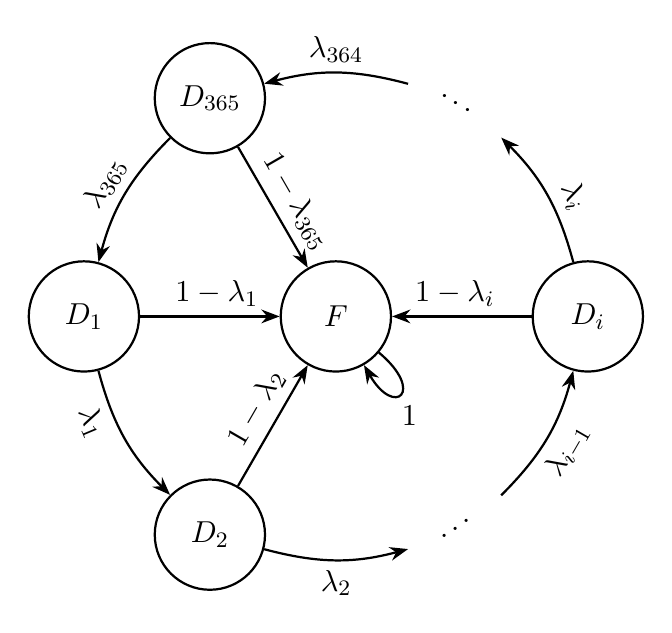
\begin{tikzpicture}[
				>=Stealth,
				state/.style={draw, circle, minimum size=14mm, line width=0.8pt},
				invisible/.style={circle, minimum size=14mm, draw=none},
				arrow/.style={->, line width=0.8pt}
				]
				
				% Centro
				\node[state, font=\fontsize{11pt}{1pt}\selectfont] (F) at (0,0) {$F$};
				
				% Hexágono
				\node[state, font=\fontsize{11pt}{1pt}\selectfont] (D1)   at (180:3.2cm) {$D_{1}$};
				\node[state, font=\fontsize{11pt}{1pt}\selectfont] (D2)   at (240:3.2cm) {$D_{2}$};
				\node[invisible, font=\fontsize{11pt}{1pt}\selectfont] (dots1) at (300:3.2cm) {};
				\node[state, font=\fontsize{11pt}{1pt}\selectfont] (Di)   at (0:3.2cm) {$D_{i}$};
				\node[invisible, font=\fontsize{11pt}{1pt}\selectfont] (dots2) at (60:3.2cm) {};
				\node[state, font=\fontsize{11pt}{1pt}\selectfont] (D365) at (120:3.2cm) {$D_{365}$};
				
				% Ciclo
				\path[arrow]
				(D1) edge[bend right=15] 
				node[font=\fontsize{11pt}{1pt}\selectfont,pos=0.3, sloped, below] {$\lambda_{1}$} (D2)
				
				(D2) edge[bend right=15] 
				node[font=\fontsize{11pt}{1pt}\selectfont,pos=0.5, sloped, below] {$\lambda_{2}$} (dots1)
				
				(dots1) edge[bend right=15]
				node[font=\fontsize{11pt}{1pt}\selectfont,pos=0.5, sloped, below] {$\lambda_{i-1}$} (Di)
				
				(Di) edge[bend right=15] 
				node[font=\fontsize{11pt}{1pt}\selectfont,pos=0.4, sloped, above] {$\lambda_{i}$} (dots2)
				
				(dots2) edge[bend right=15]
				node[font=\fontsize{11pt}{1pt}\selectfont,pos=0.5, sloped, above] {$\lambda_{364}$} (D365)
				
				(D365) edge[bend right=15] 
				node[font=\fontsize{11pt}{1pt}\selectfont,pos=0.5, sloped, above] {$\lambda_{365}$} (D1);
				
				% Hacia F
				\path[arrow]
				(D1) edge node[font=\fontsize{11pt}{1pt}\selectfont,pos=0.55,above] {$1-\lambda_{1}$} (F)
				(D2) edge node[font=\fontsize{11pt}{1pt}\selectfont,pos=0.55, sloped, above] {$1-\lambda_{2}$} (F)
				(Di) edge node[font=\fontsize{11pt}{1pt}\selectfont,pos=0.55, above] {$1-\lambda_{i}$} (F)
				(D365) edge node[font=\fontsize{11pt}{1pt}\selectfont,pos=0.55, sloped, above] {$1-\lambda_{365}$} (F);
				
				% Loop
				\path[arrow]
				(F) edge[
				loop,
				out=320, 
				in=300,
				looseness=8
				] node[font=\fontsize{11pt}{1pt}\selectfont,pos=0.8, xshift=10pt, yshift=-10pt] {$1$} (F);
				
				% Puntos suspensivos
				\node[font=\fontsize{11pt}{1pt}\selectfont, rotate=35] at (300:3.1cm) {$\cdots$};
				\node[font=\fontsize{11pt}{1pt}\selectfont, rotate=-30] at (60:3.1cm) {$\cdots$};
				
			\end{tikzpicture}
		}





\section*{Methodology}%


\iffalse
\begin{center}
\begin{figure}
    \captionsetup{type=figure}
    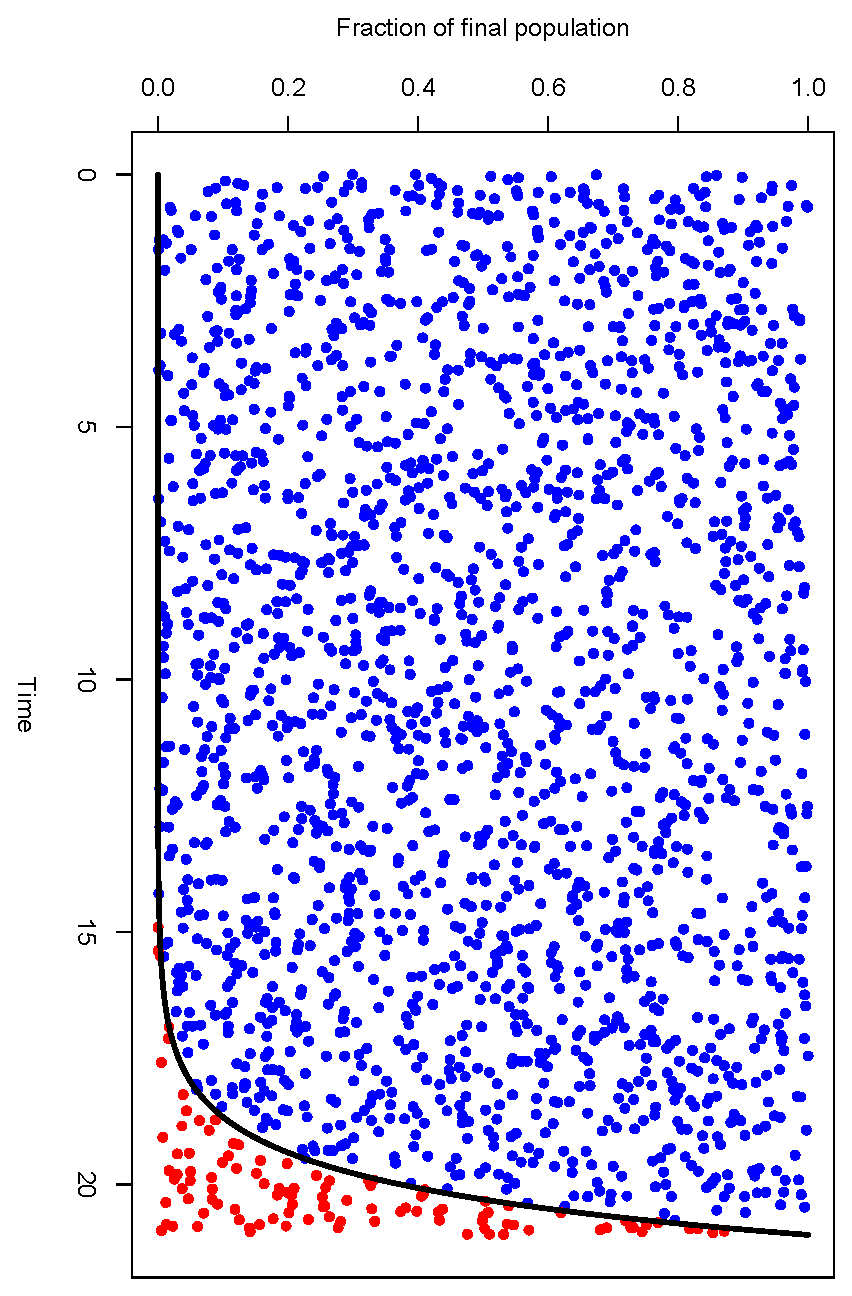
\includegraphics[height=0.305\textwidth,angle=90]{images/Graphical-Poster.eps}
    \caption{Acceptance-rejection method.}
    \label{fig:metodo_grafico}               
\end{figure}
\end{center}
\fi

\vspace{-1cm}\section*{Results}%


\begin{figure}
	\centering
	\subfloat[
	\centering $p$-value of Kolmogorov-Smirnov test at different population sizes.
	]{
		\hspace{-1.5cm}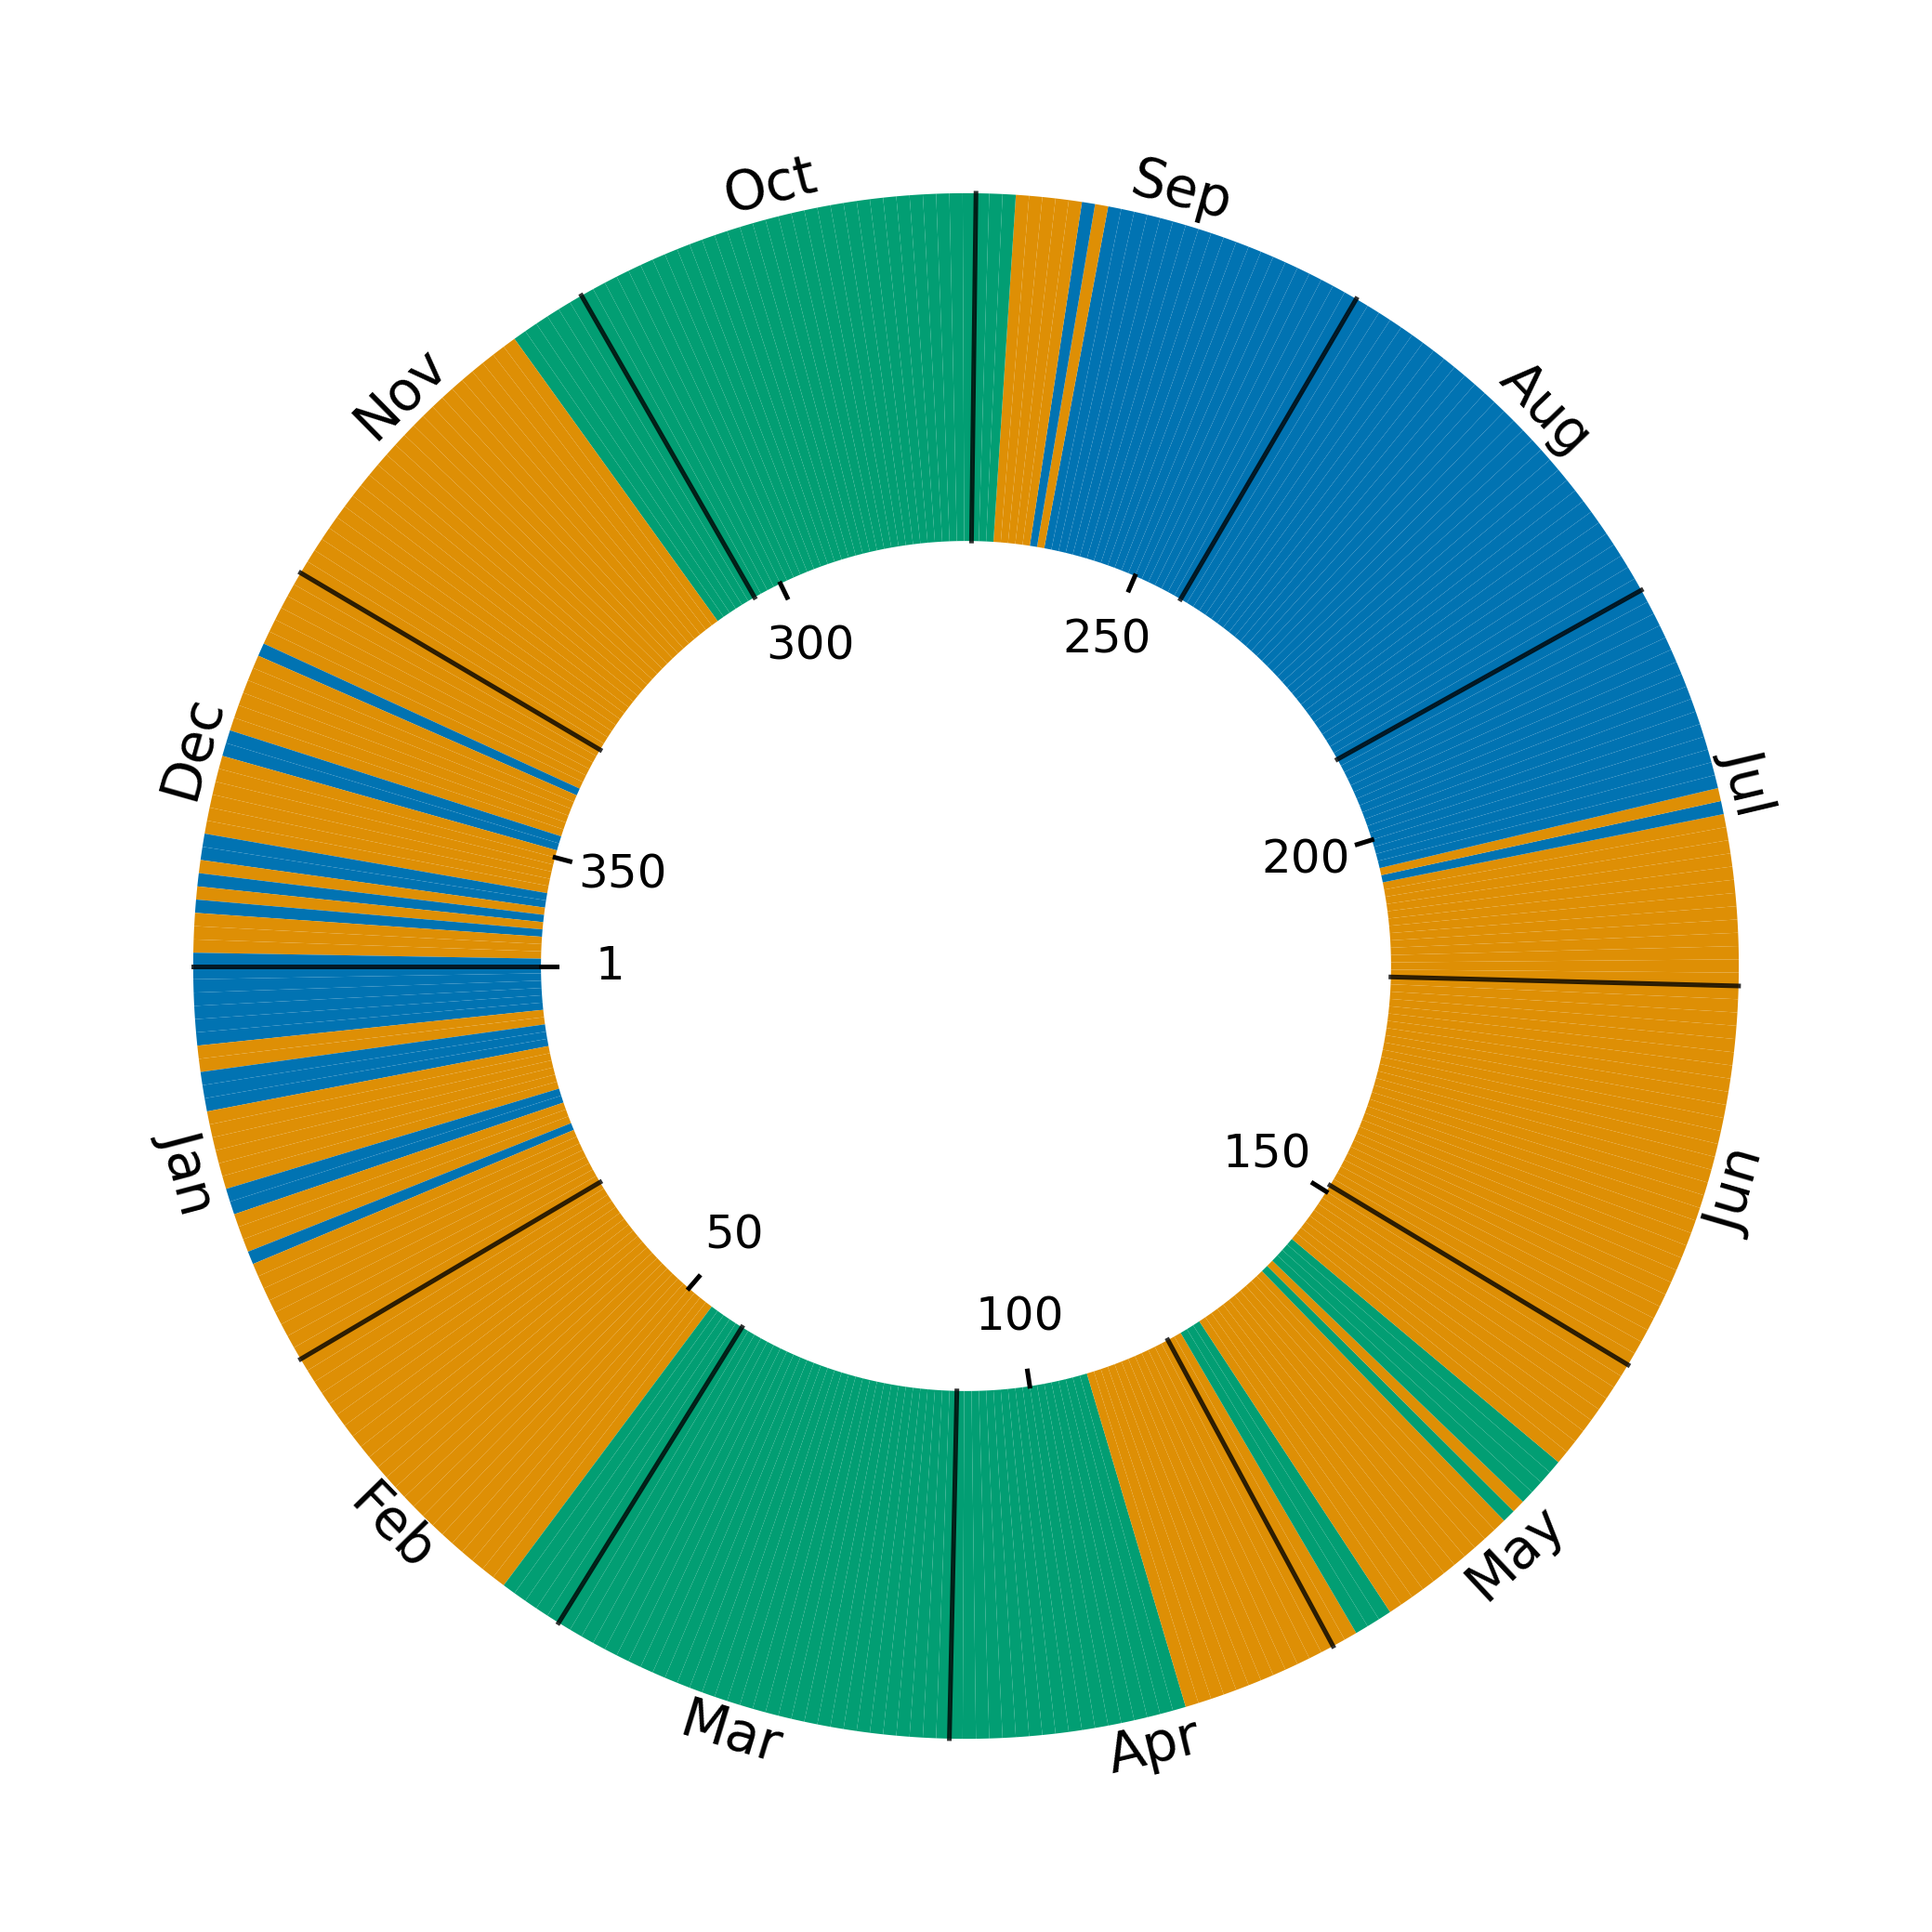
\includegraphics[
		width=0.28\textwidth
		]{images/[Brandenburg][Circular][Euclidean]NO_CI.png}
	}
	\subfloat[
	\centering $\chi^2$ goodness-of-fit for Luria-Delbruck distribution.
	]{
		\hspace{-3cm}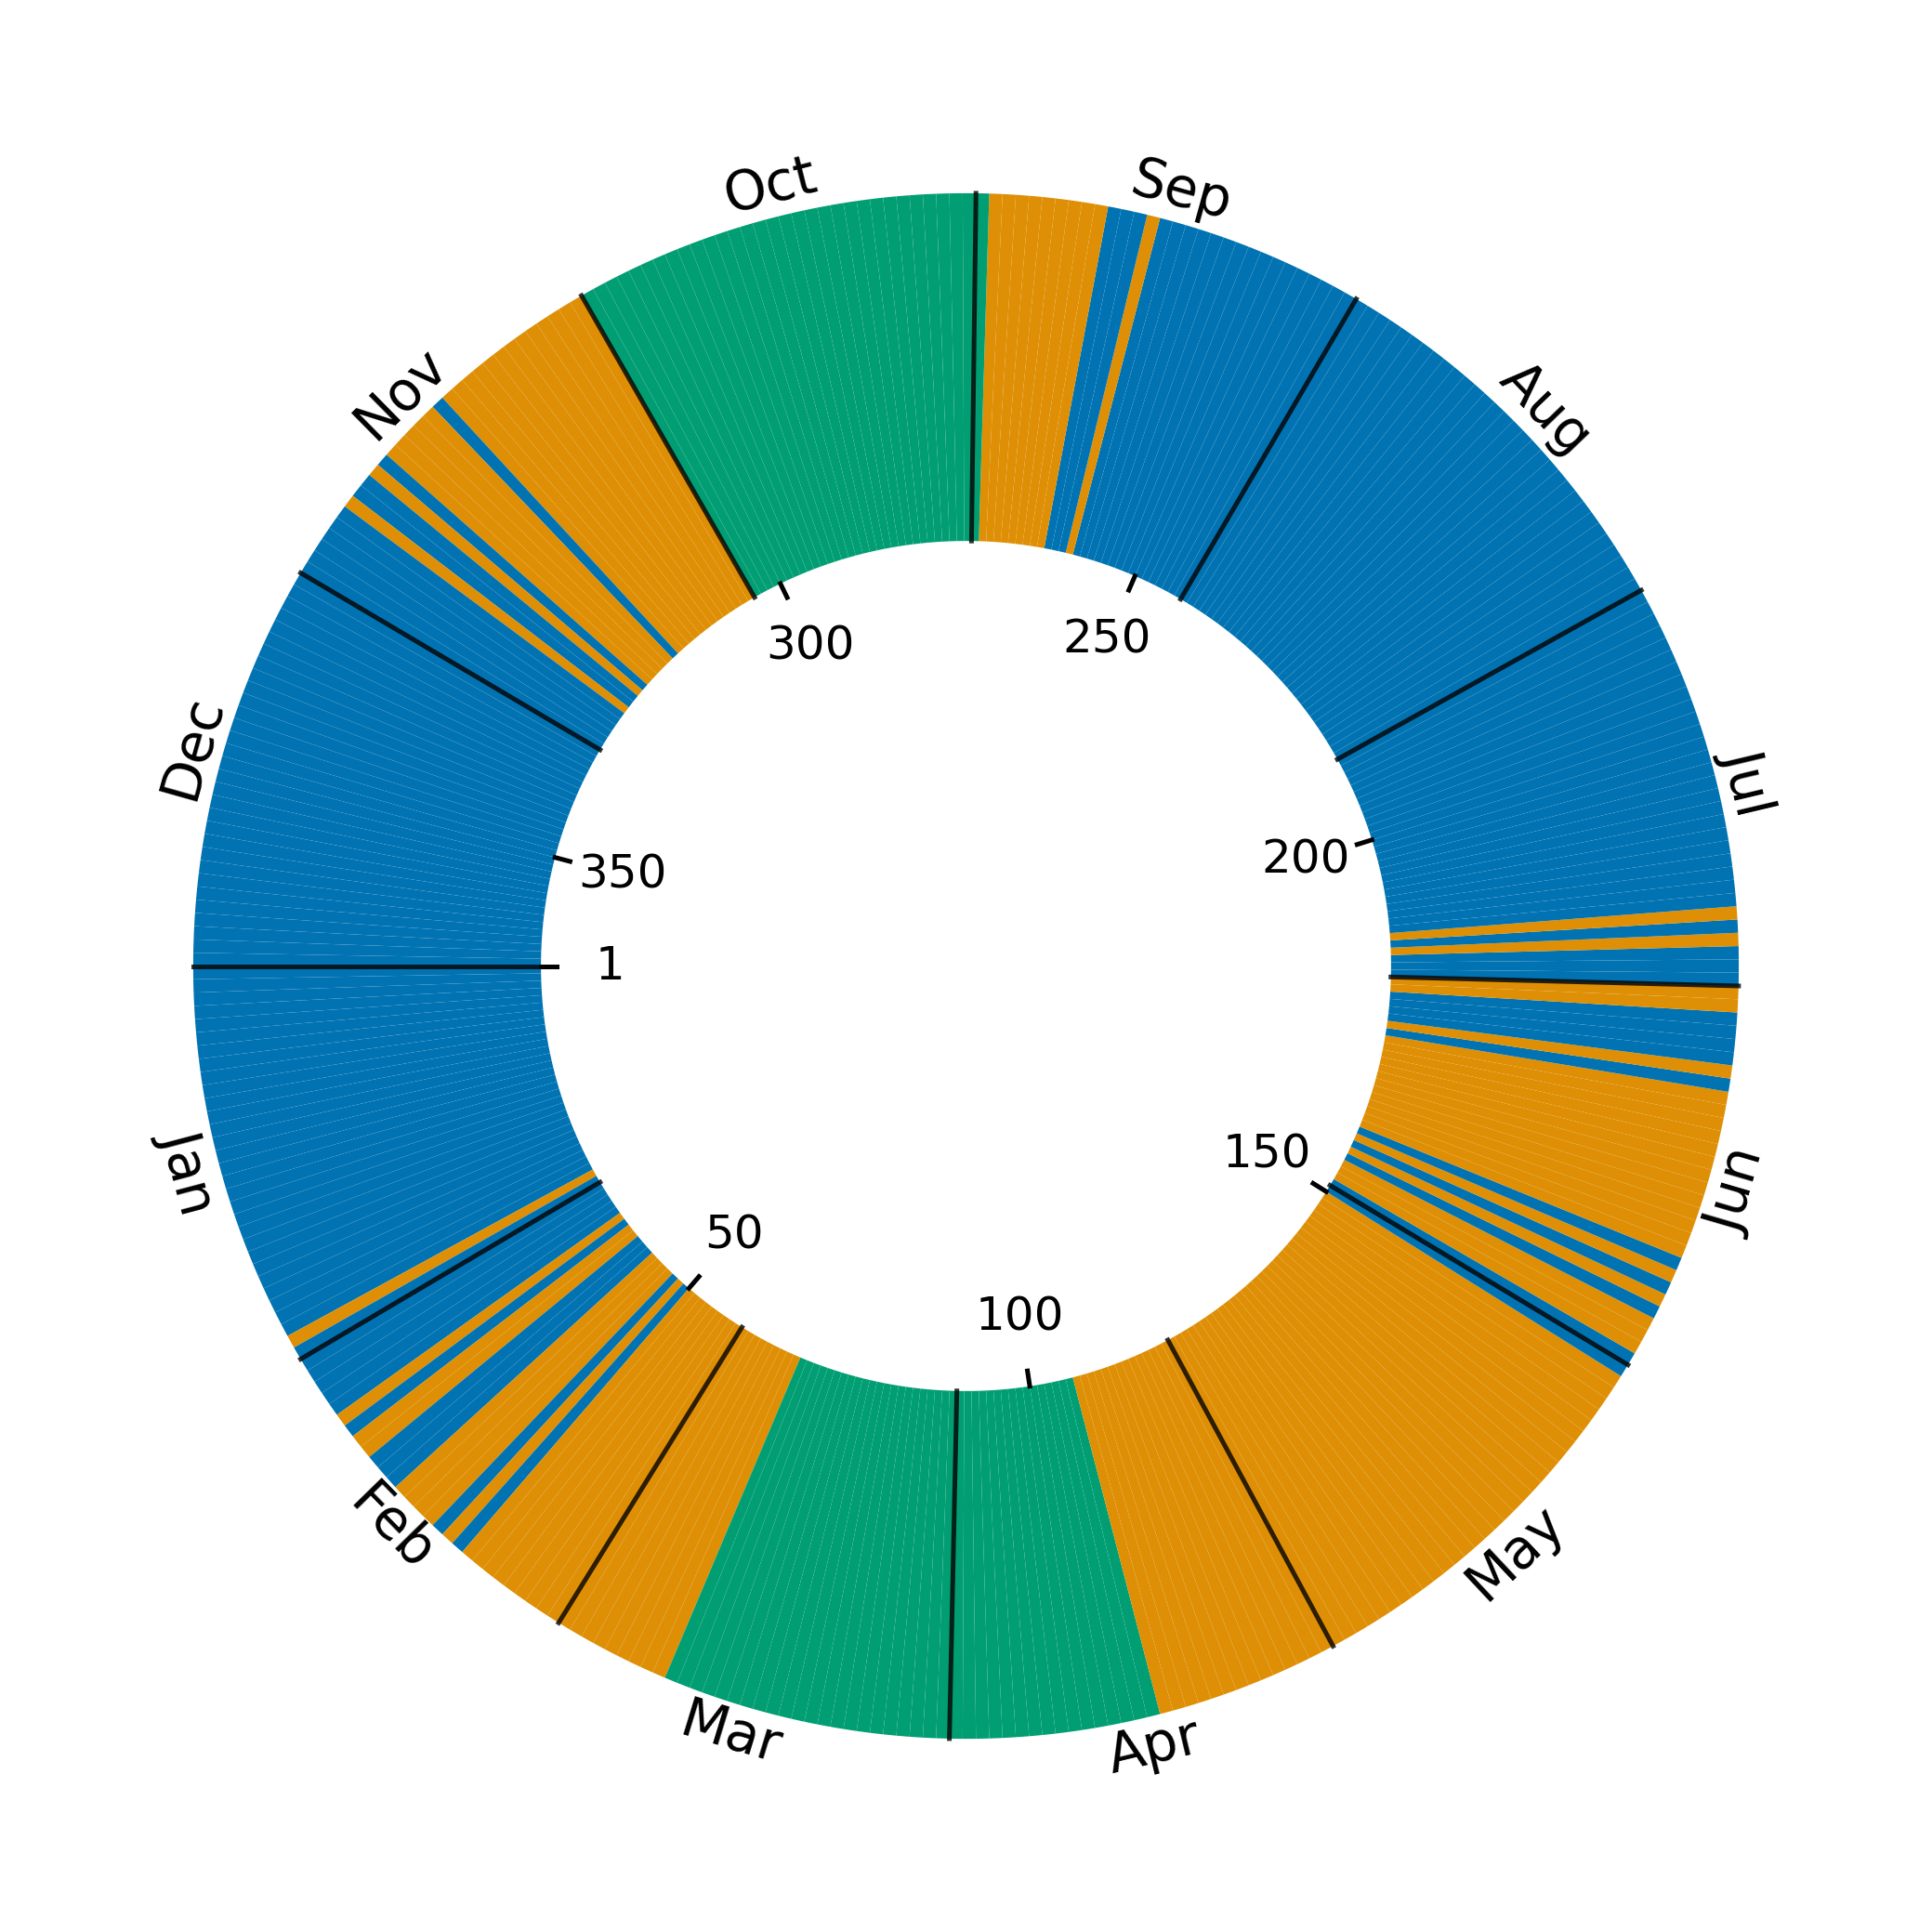
\includegraphics[
		width=0.28\textwidth
		]{images/[Brandenburg][Circular][Manhattan]NO_CI.png}
	}
	
	\caption{Statistical comparisons.}
	\label{fig:KS_test}
\end{figure}


\begin{figure}
	\centering
	\subfloat[
	\centering $p$-value of Kolmogorov-Smirnov test at different population sizes.
	]{
		\hspace{-1.5cm}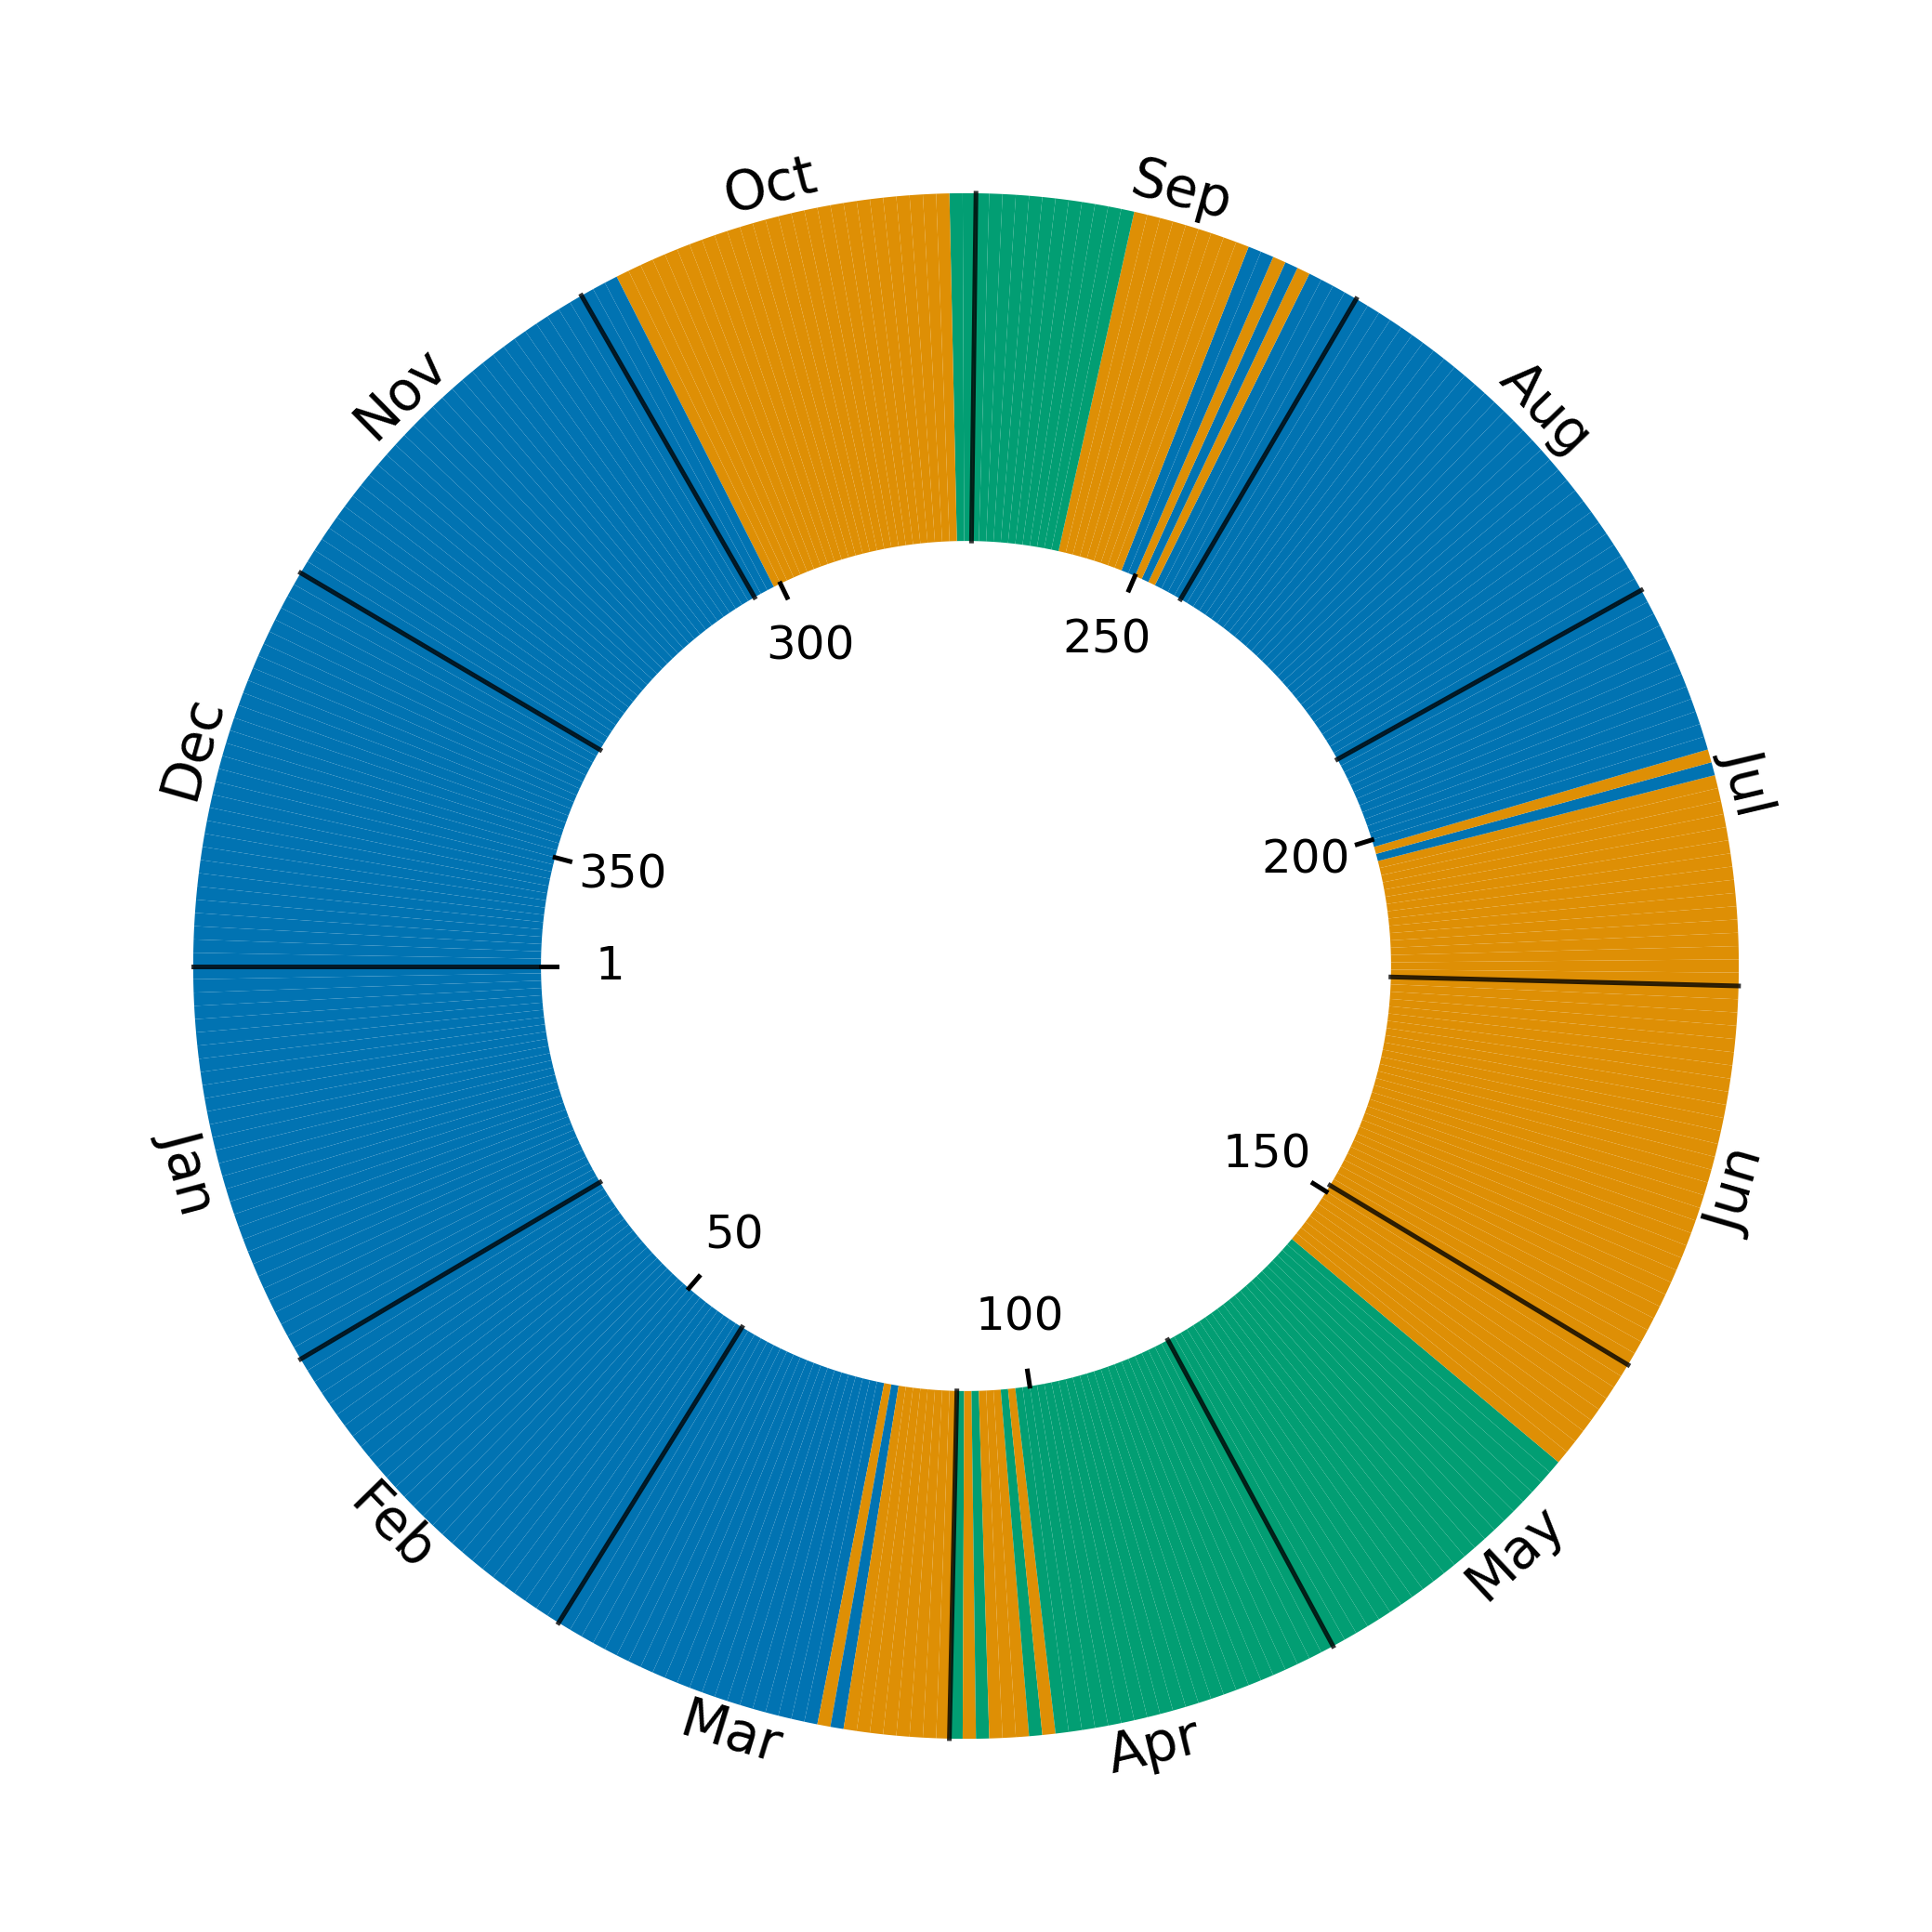
\includegraphics[
		width=0.28\textwidth
		]{images/[Saxony][Circular][Euclidean]NO_CI.png}
	}
	\subfloat[
	\centering $\chi^2$ goodness-of-fit for Luria-Delbruck distribution.
	]{
		\hspace{-3cm}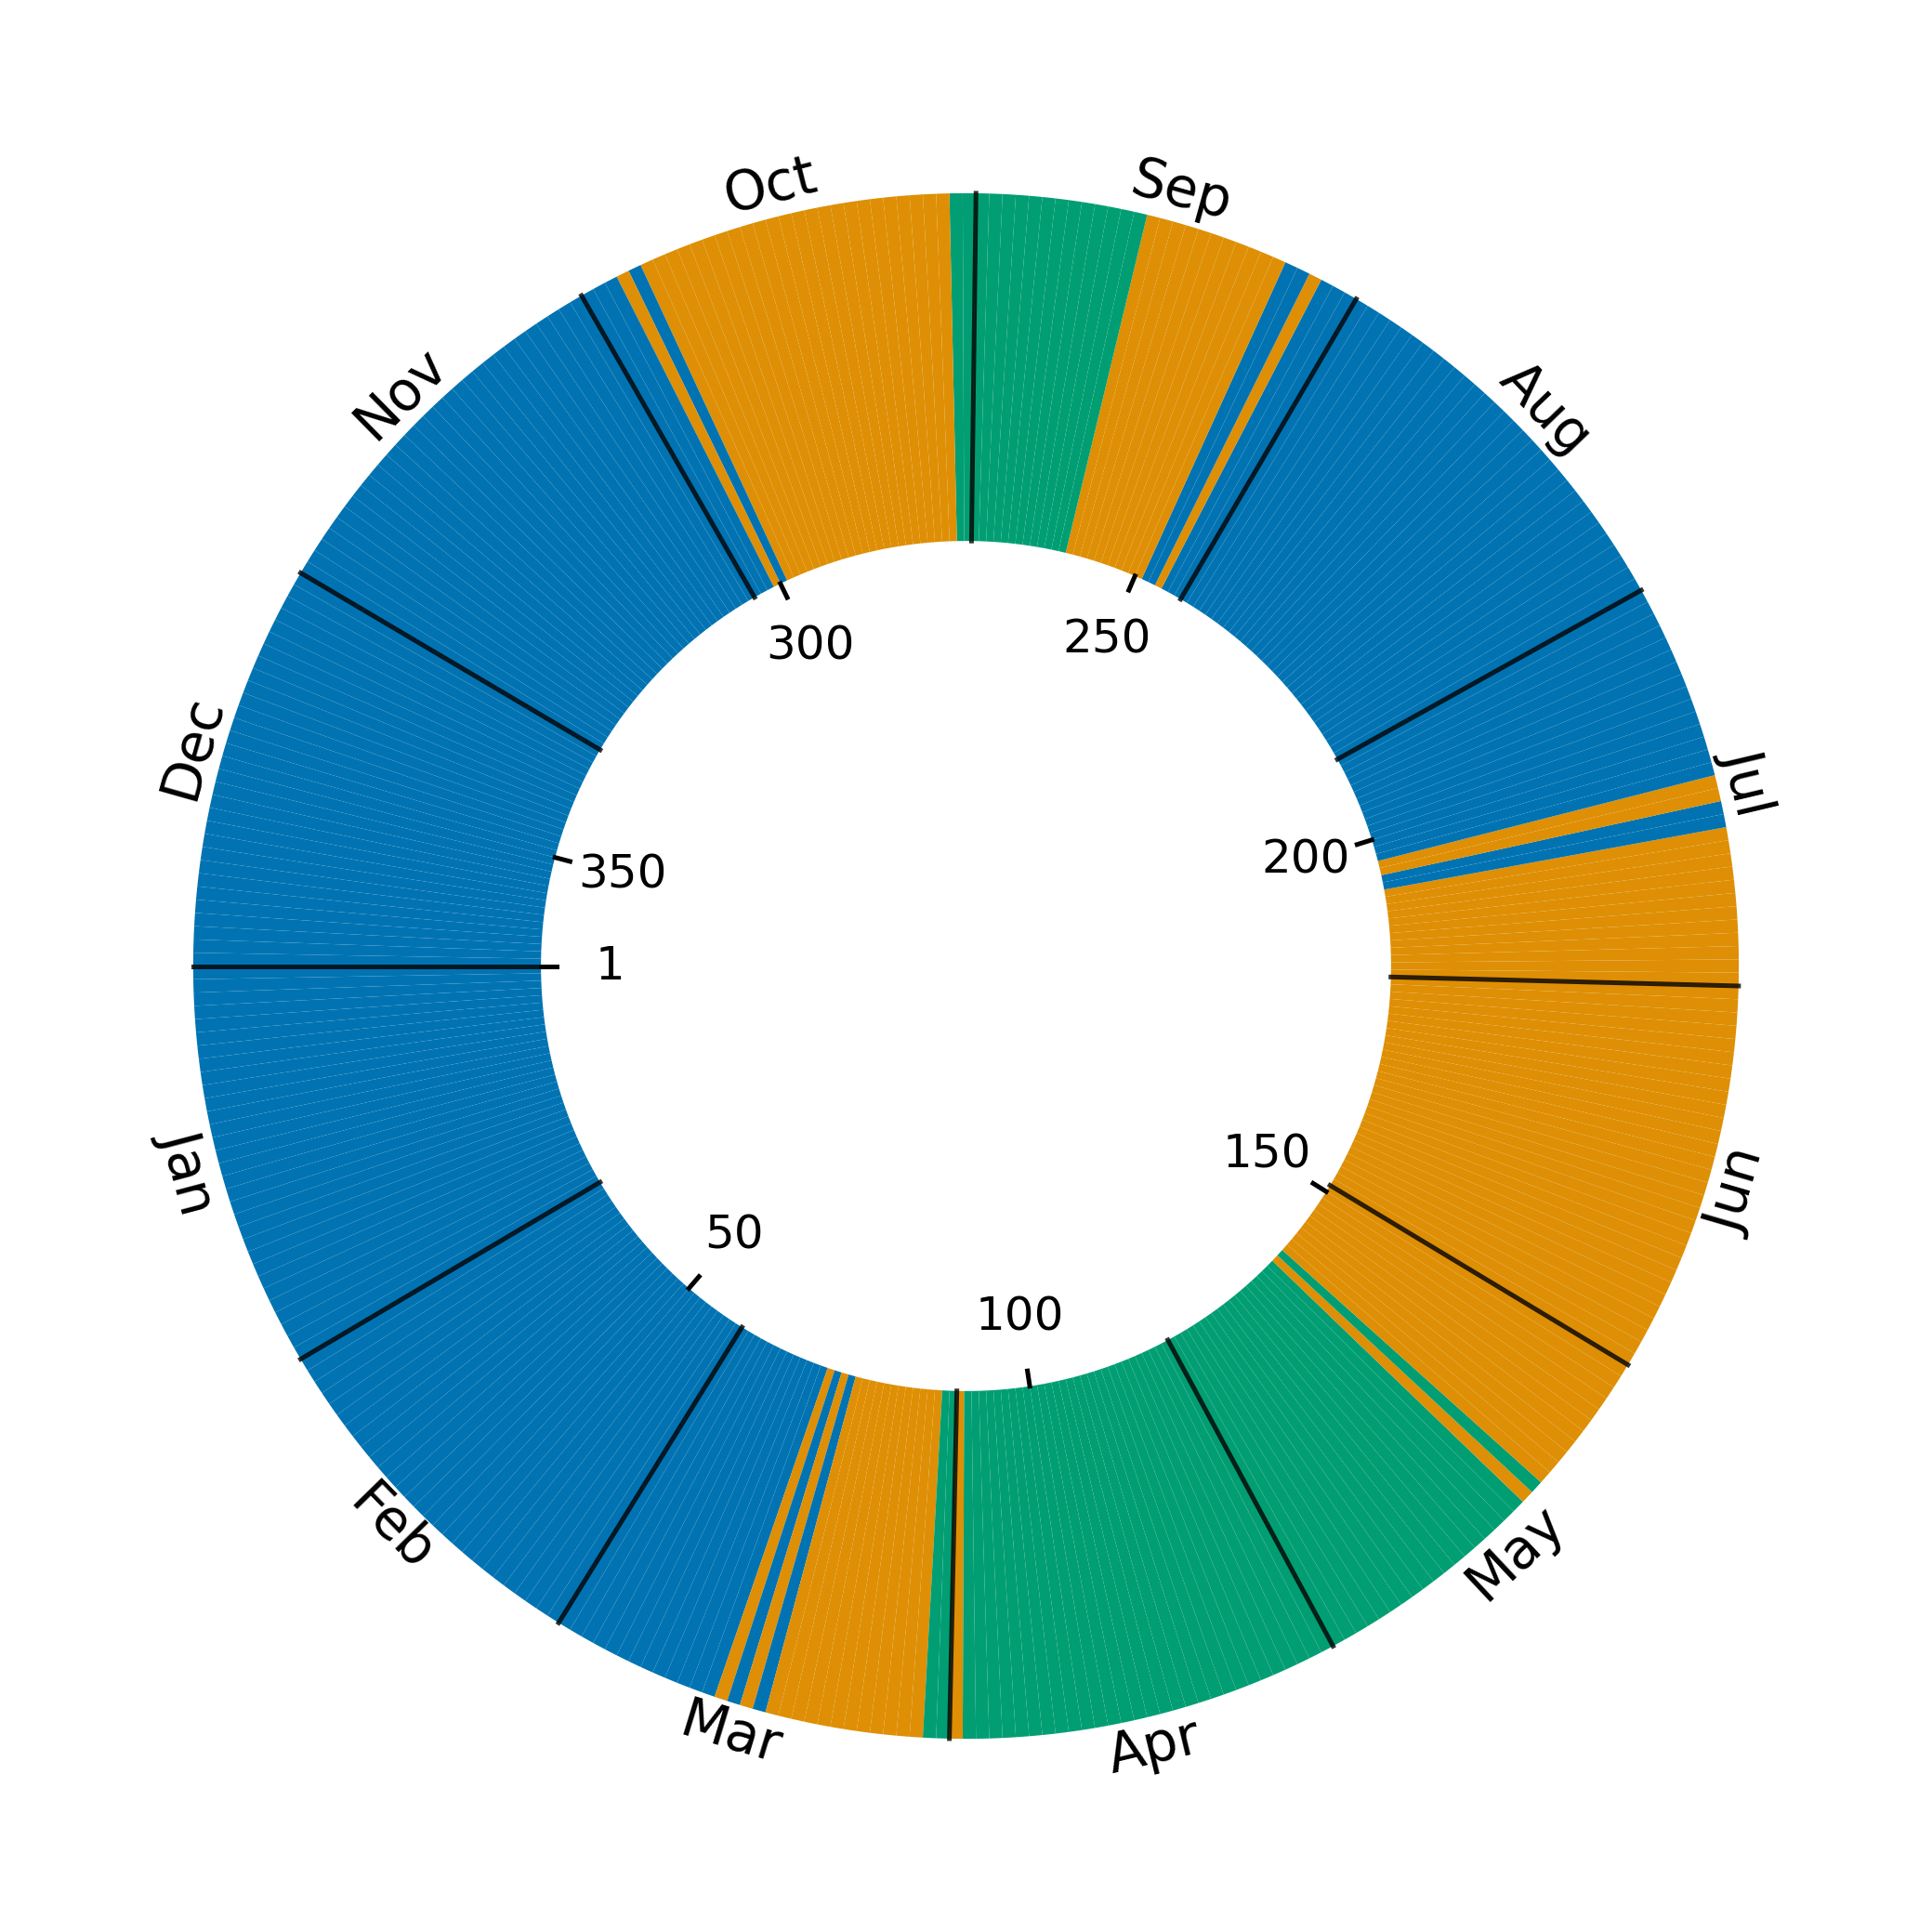
\includegraphics[
		width=0.28\textwidth
		]{images/[Saxony][Circular][Manhattan]NO_CI.png}
	}
	
	\caption{Statistical comparisons.}
	\label{fig:KS_test}
\end{figure}

\begin{figure}
	\centering
	\subfloat[
	\centering $p$-value of Kolmogorov-Smirnov test at different population sizes.
	]{
		\hspace{-1.5cm}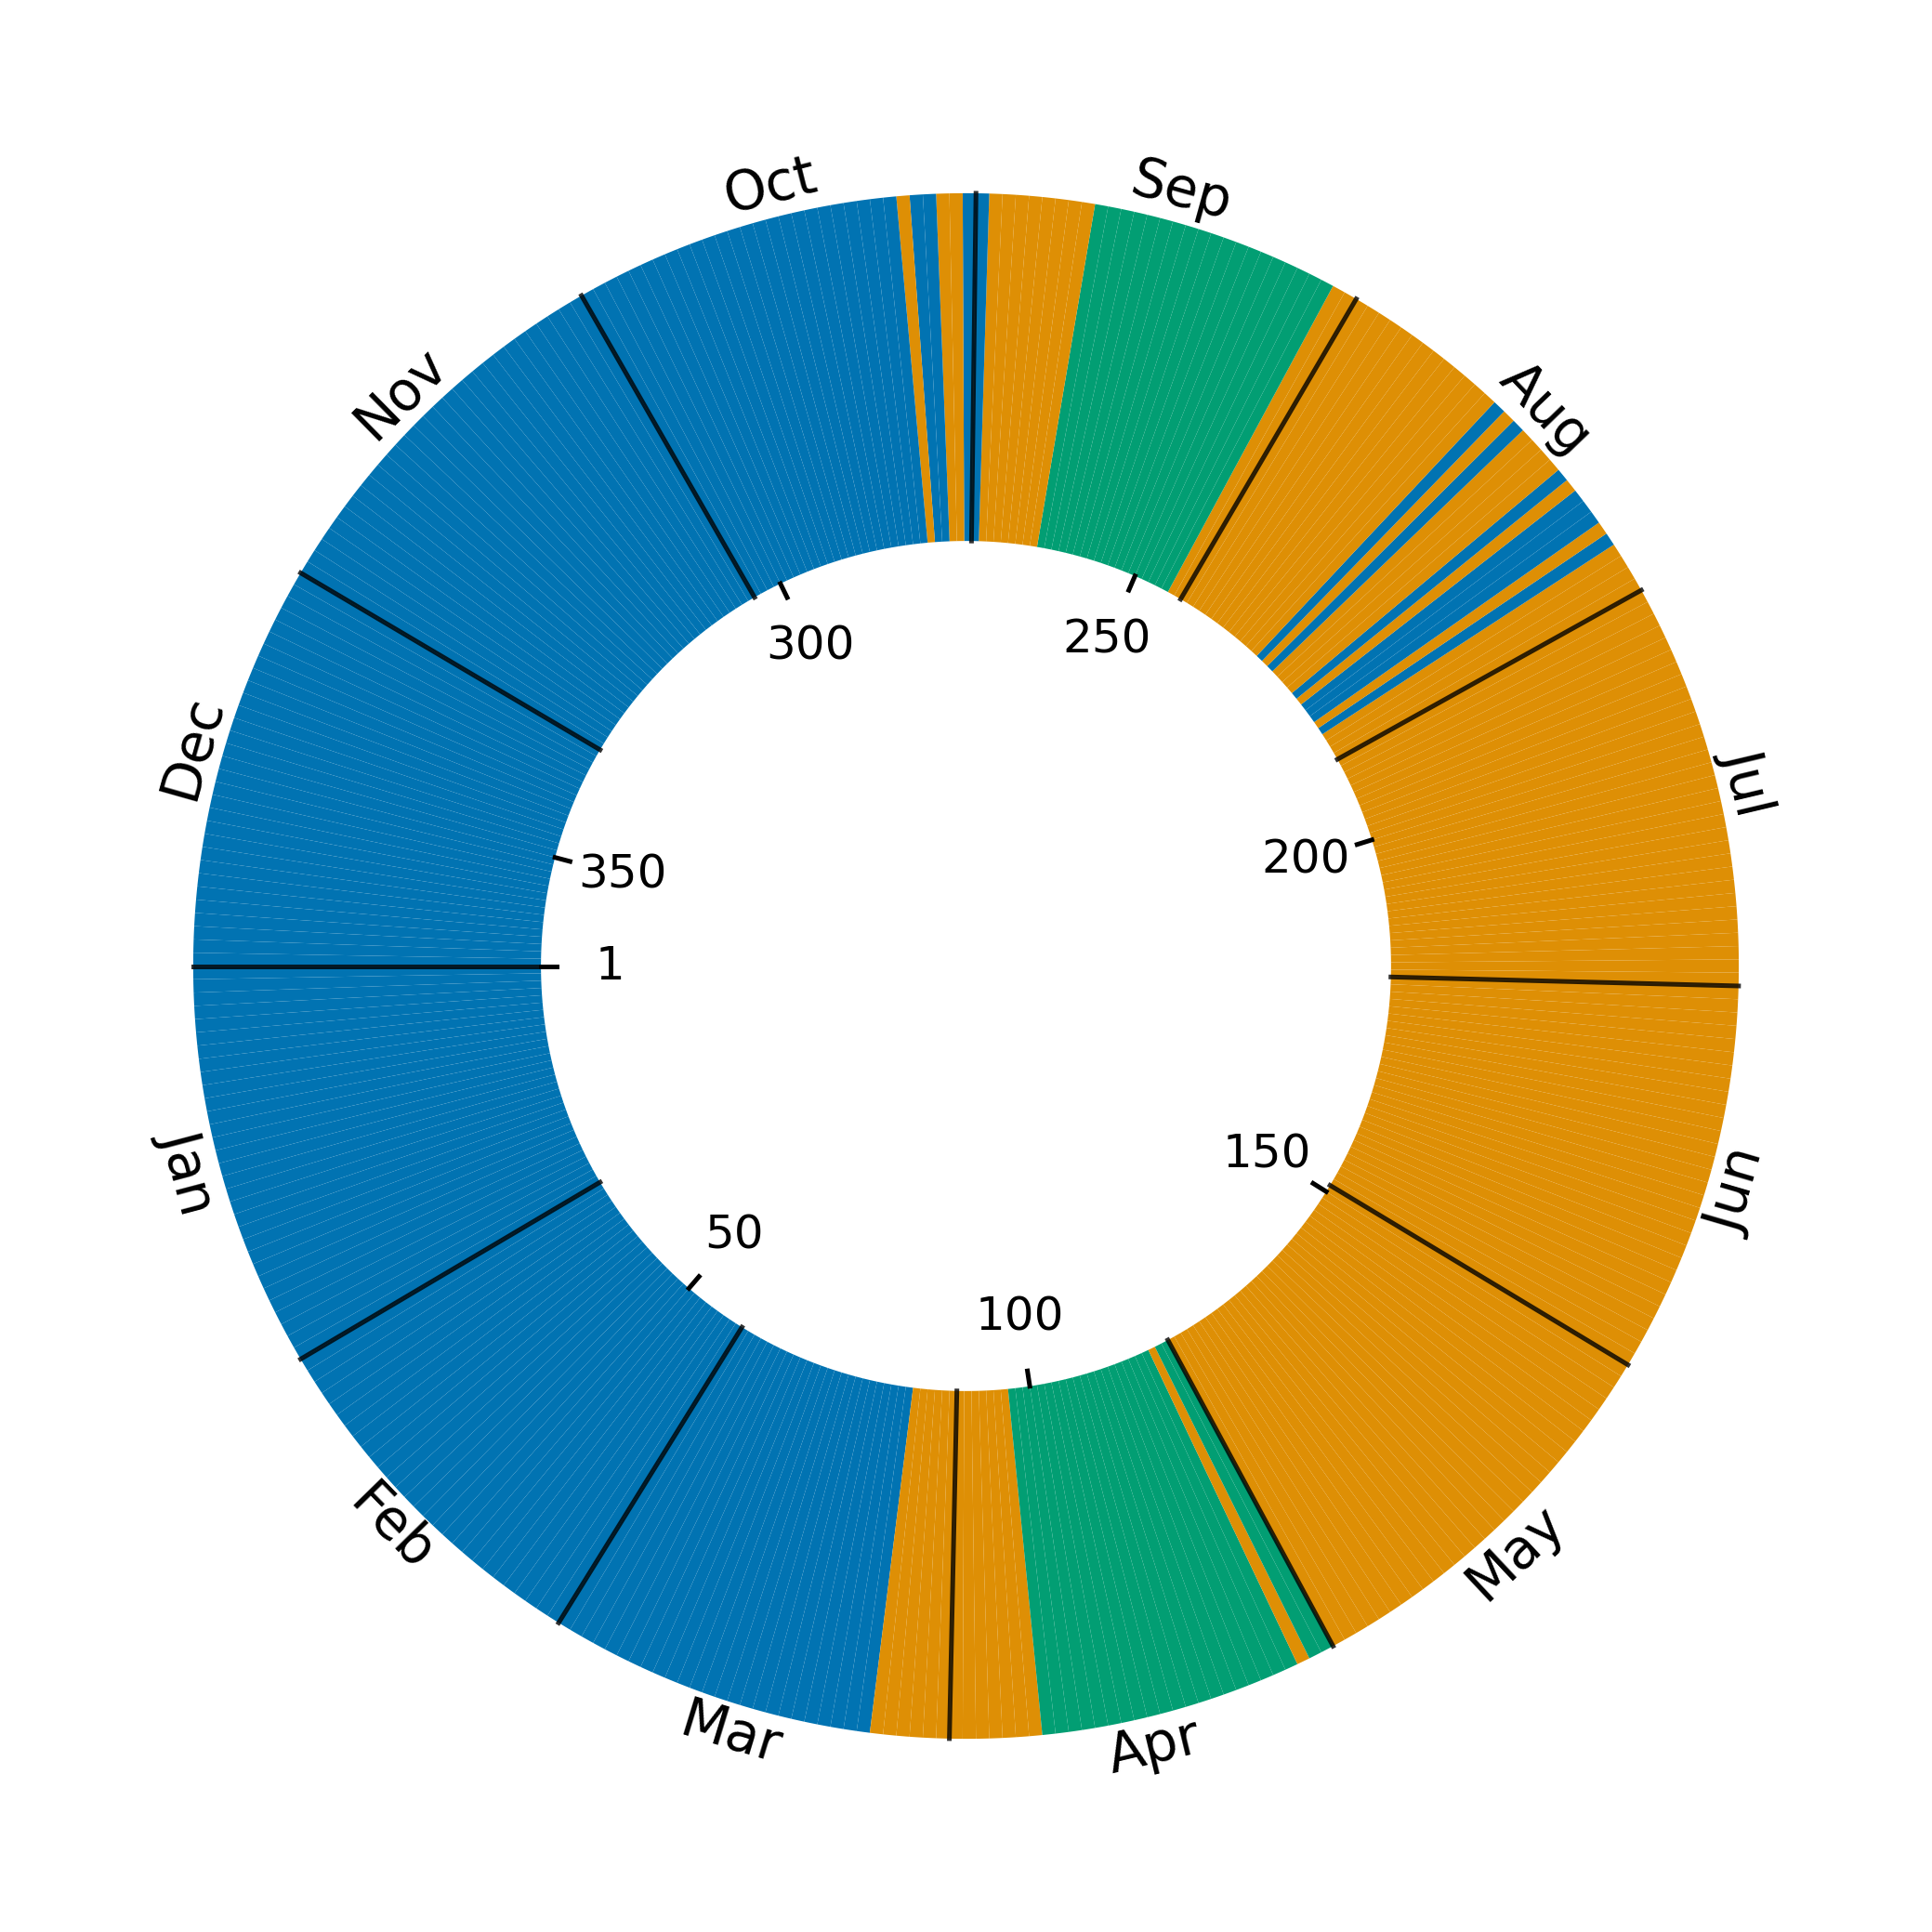
\includegraphics[
		width=0.28\textwidth
		]{images/[Bavaria][Circular][Euclidean]NO_CI.png}
	}
	\subfloat[
	\centering $\chi^2$ goodness-of-fit for Luria-Delbruck distribution.
	]{
		\hspace{-3cm}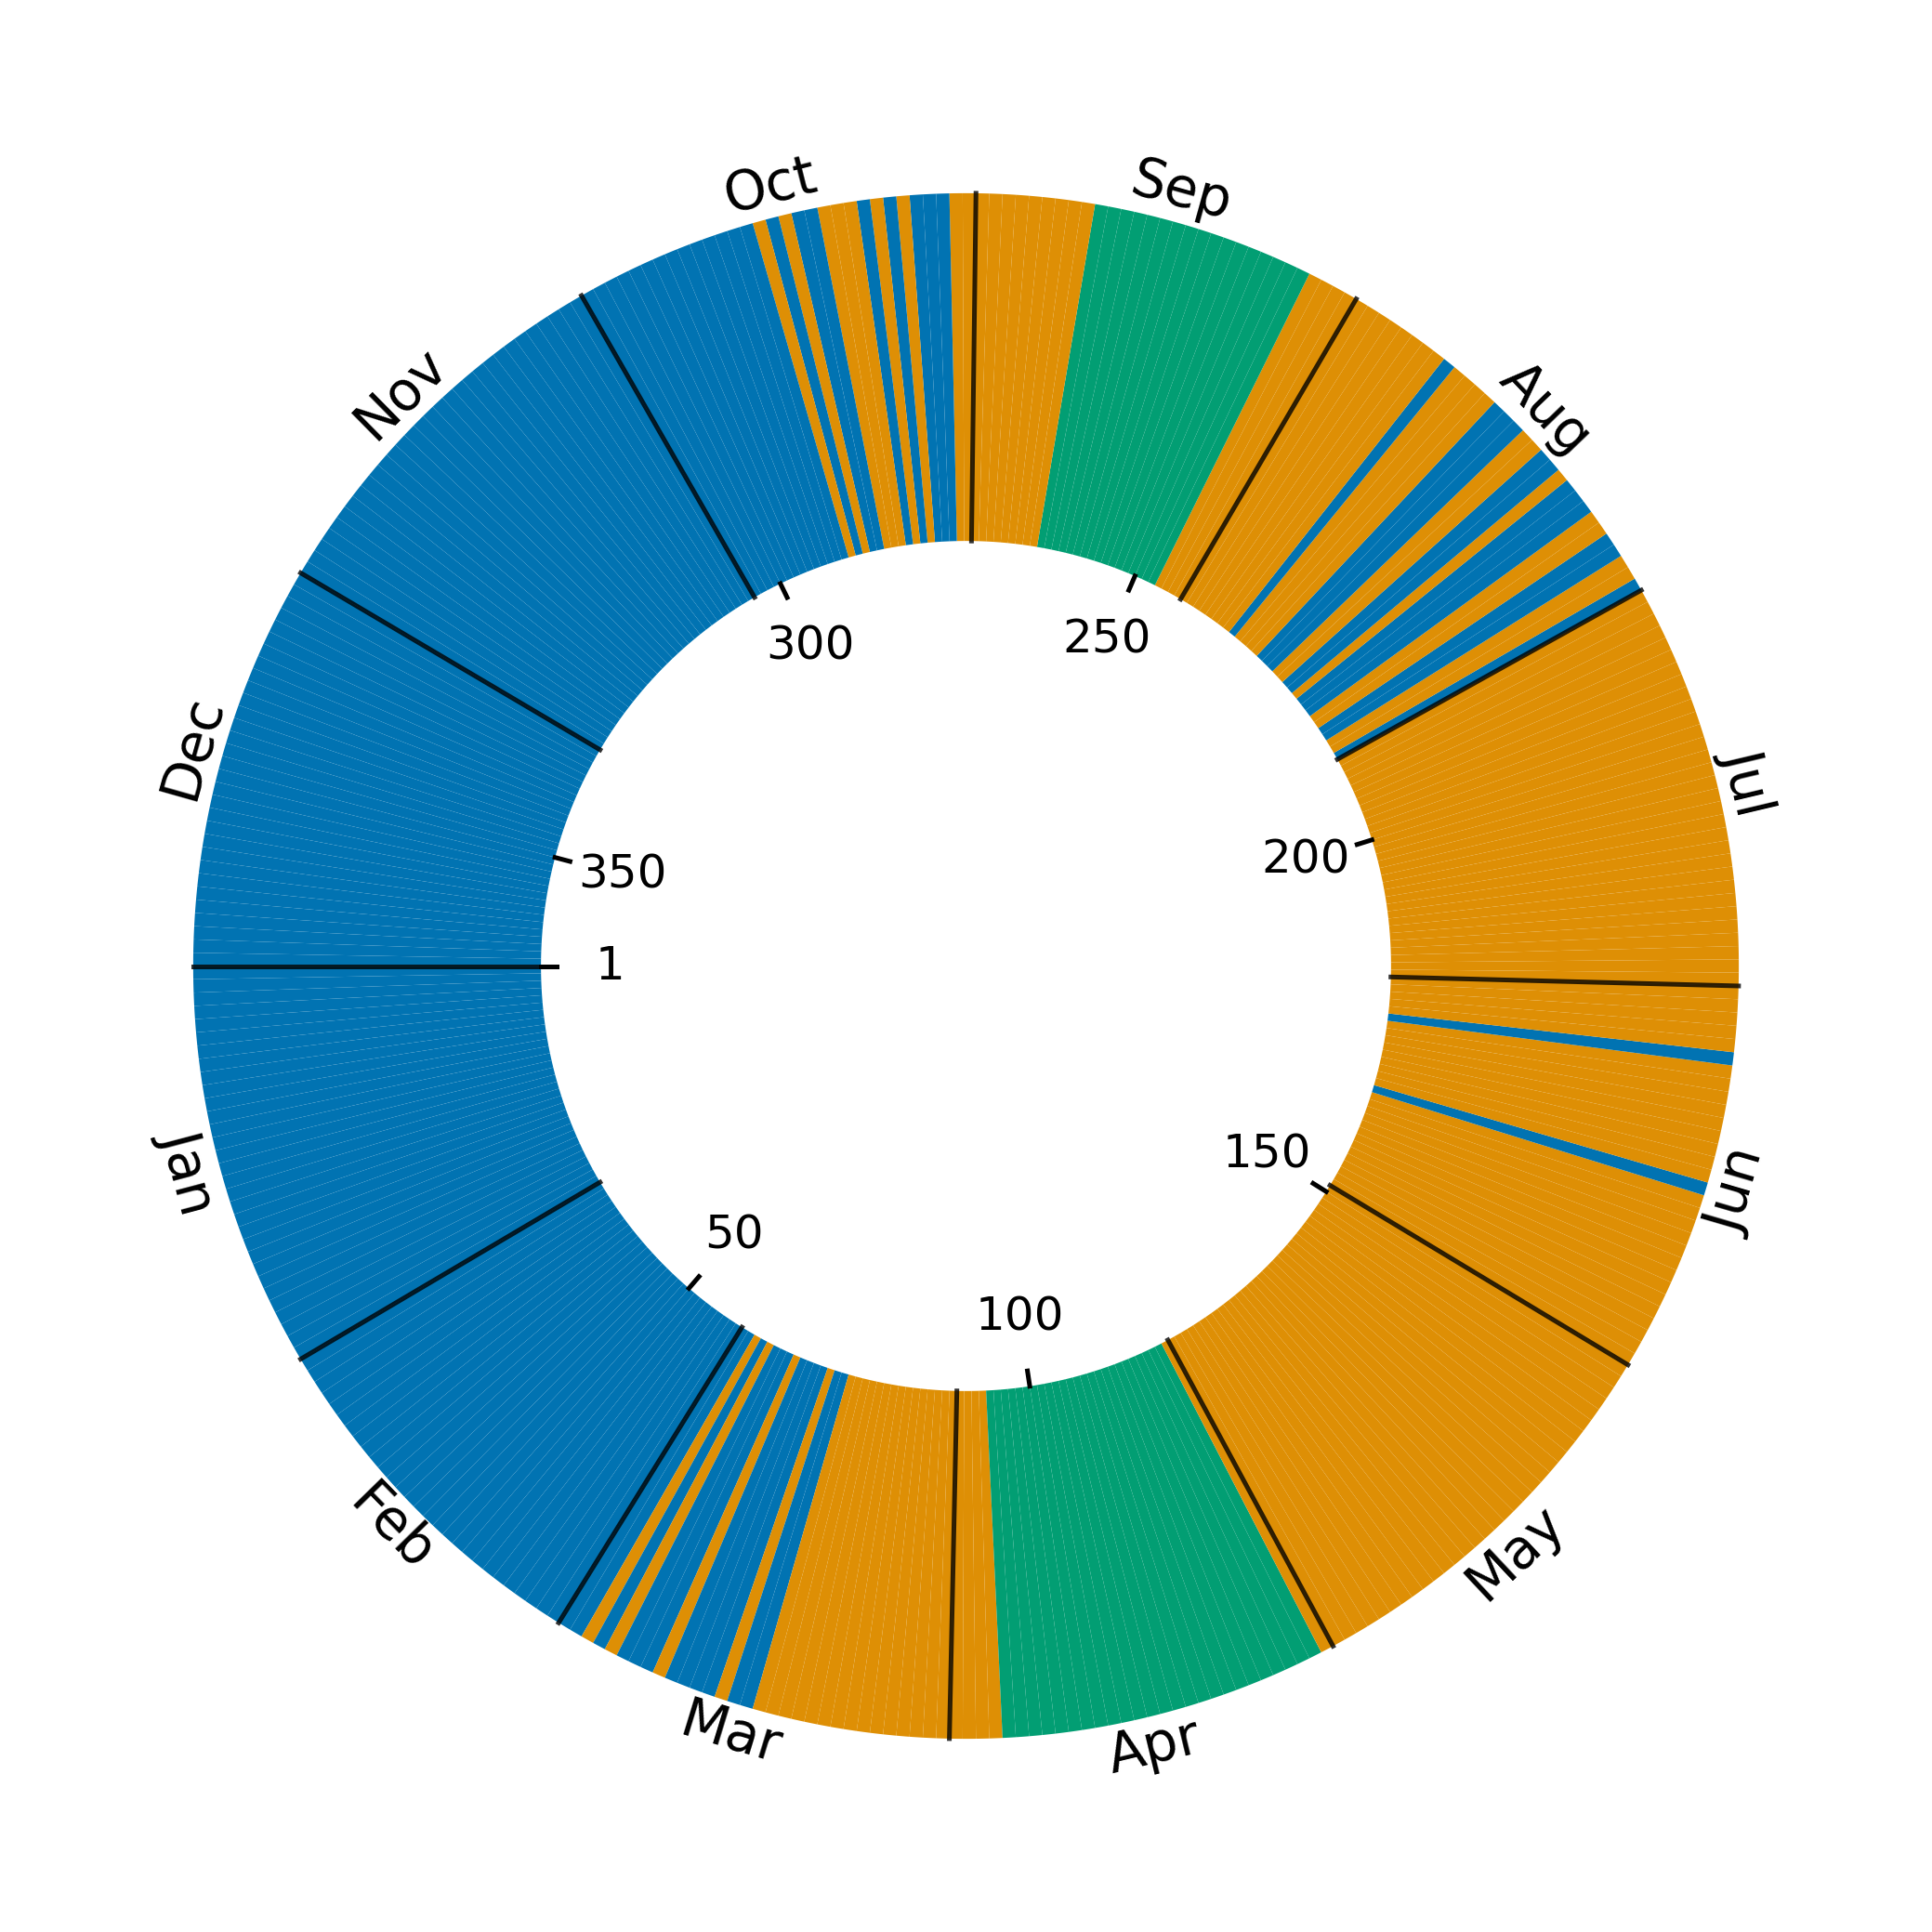
\includegraphics[
		width=0.28\textwidth
		]{images/[Bavaria][Circular][Manhattan]NO_CI.png}
	}
	
	\caption{Statistical comparisons.}
	\label{fig:KS_test}
\end{figure}



\iffalse
\begin{center} 
\begin{figure}%
    \centering
    \subfloat[\centering Histogram of the number of mutator cells.]{\hspace{-1cm}{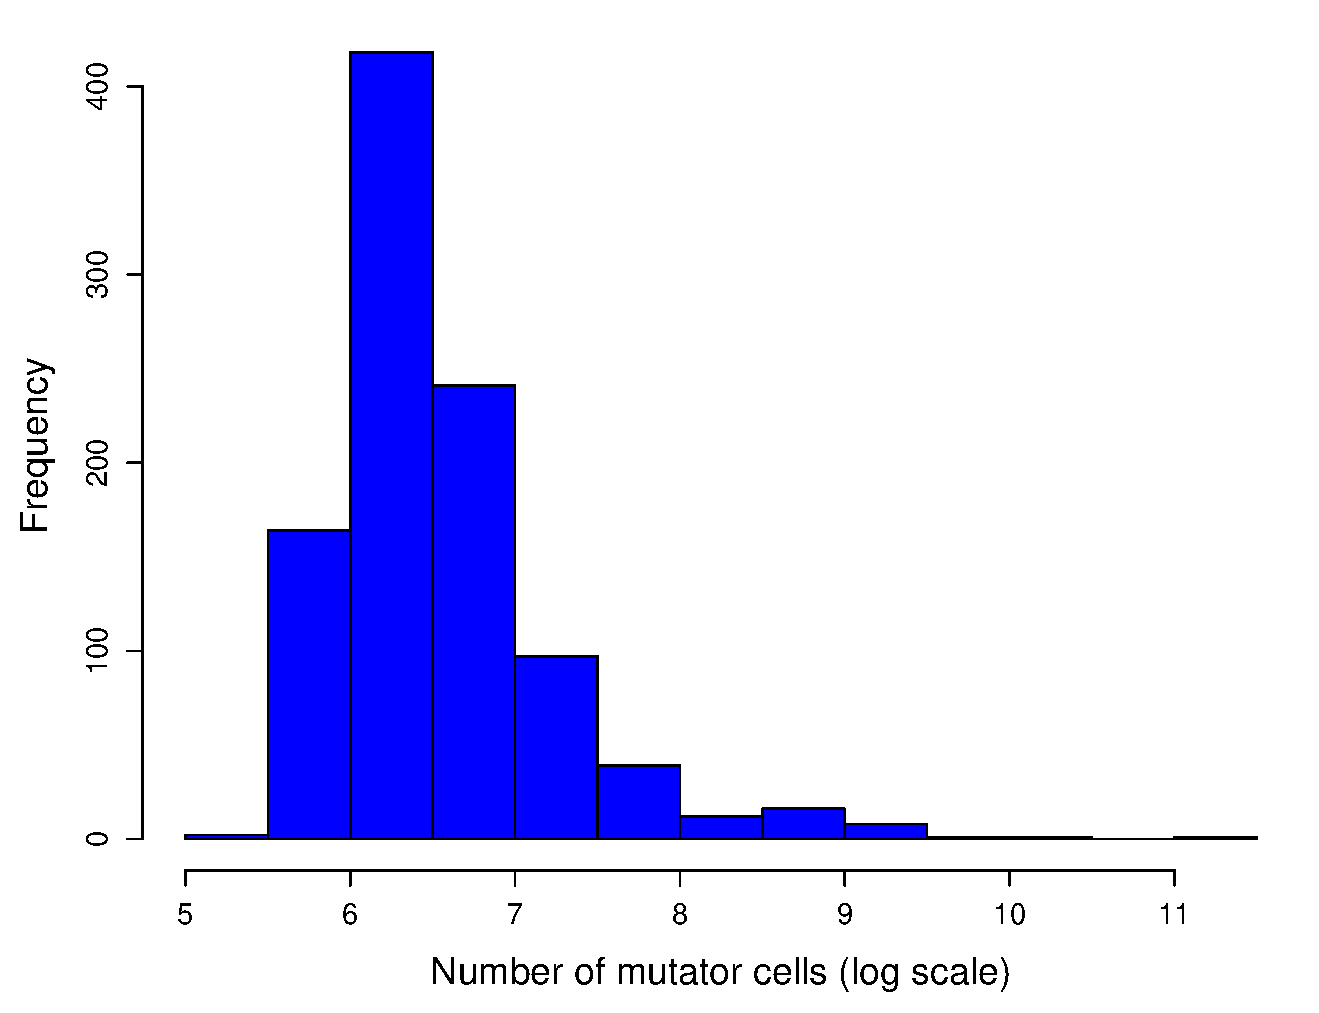
\includegraphics[width=0.248\textwidth]{images/Hist-Mutators.eps} \label{LD_dist}}}%
    %\qquad
    \subfloat[\centering Histogram of the number of mutant cells with mutator phenotypes.]{{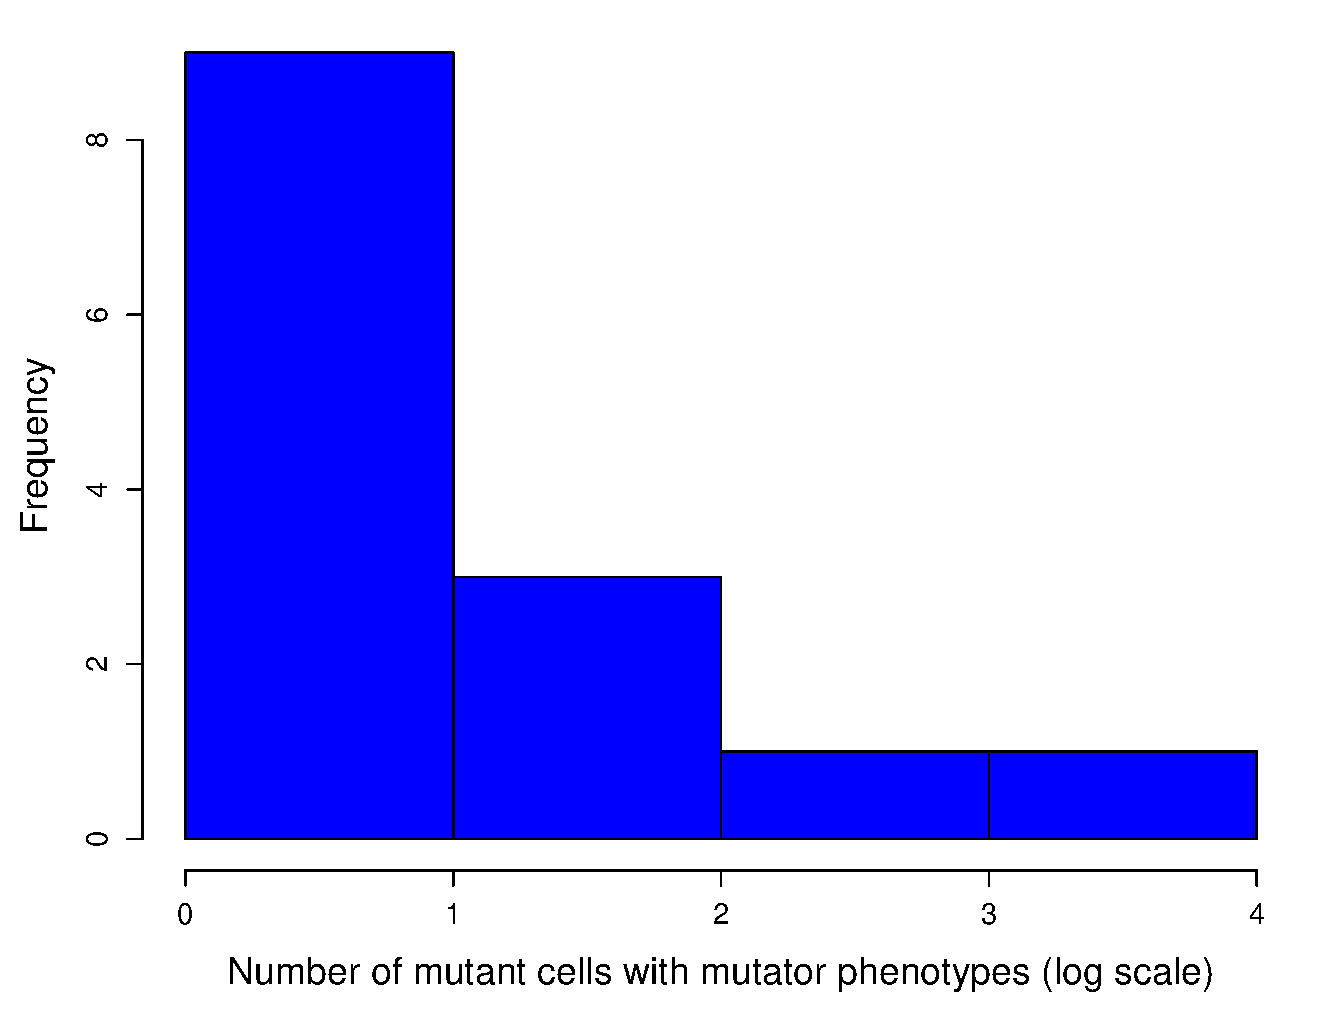
\includegraphics[width=0.25\textwidth]{images/Hist-Mutants-Mutator-Phenotype.eps} }}%
    \caption{\centering Histograms of 100 simulations.}%
    \label{fig:KS_test}%
\end{figure}
\end{center}
\fi        


        \iffalse
        \begin{figure}
            \centering
            \captionsetup{type=figure}
            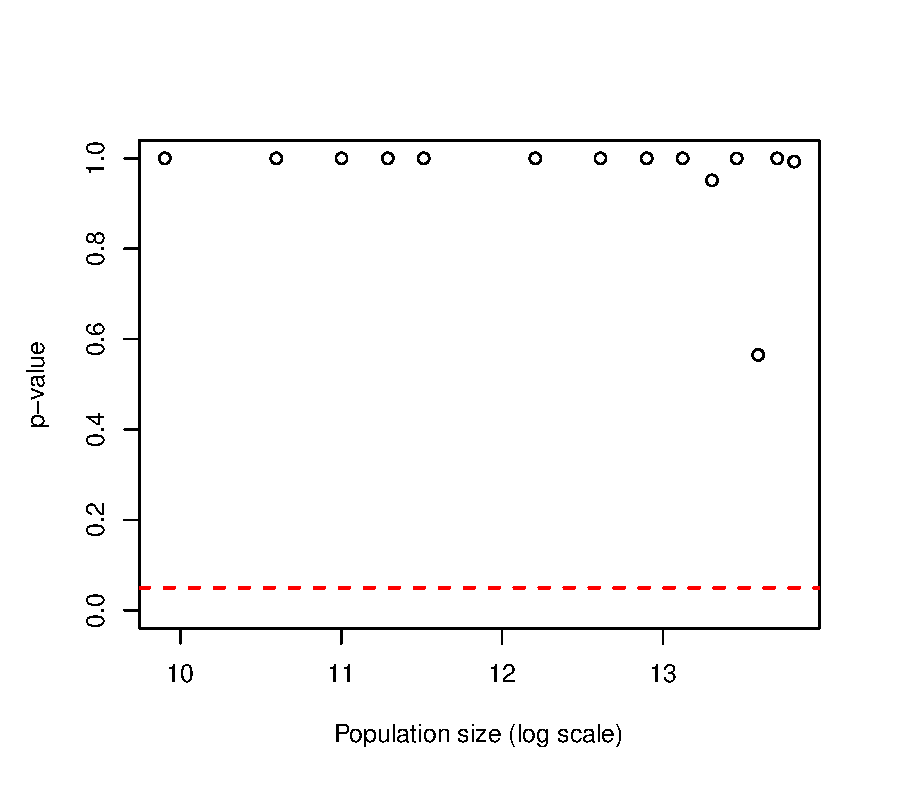
\includegraphics[scale=1]{images/Comparative_Moran_GM_p_value.eps}
            \caption{Example of a figure.}
            \label{fig:p_value}
        \end{figure}
        \begin{figure}
            \centering
            \captionsetup{type=figure}
            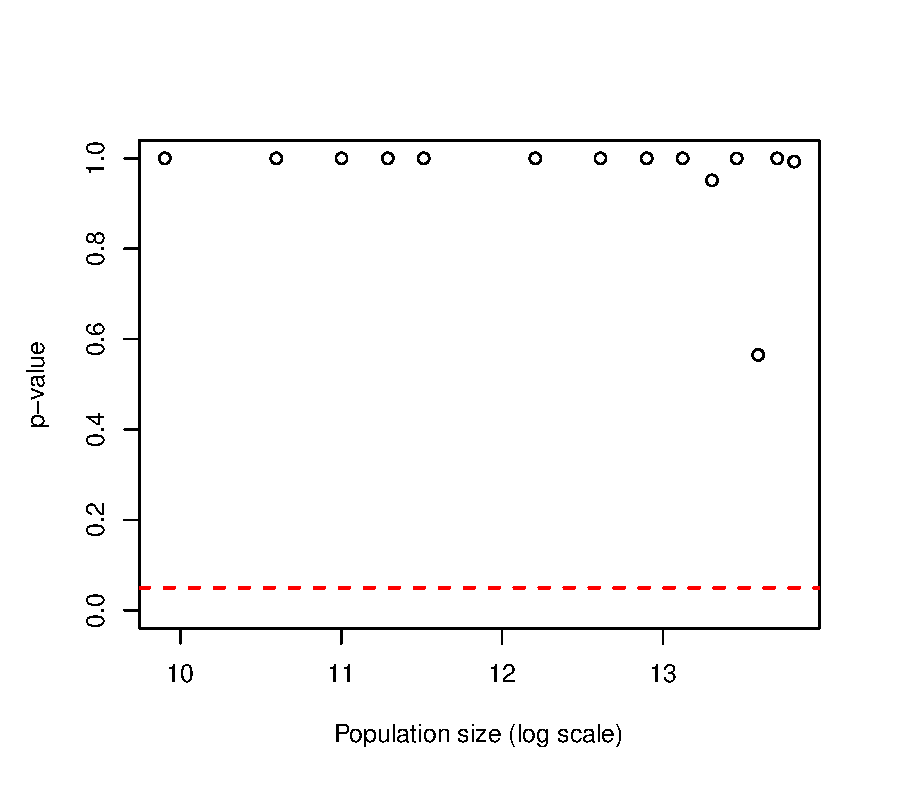
\includegraphics[scale=1]{images/Comparative_Moran_GM_p_value.eps}
            \caption{Example of a figure.}
            \label{fig:D_Statistic}
        \end{figure}
    \fi
\iffalse                
    
            \begin{figure}
                \centering
                \captionsetup{type=figure}
                \includegraphics[scale=1.5]{example-image-b}
                \caption{Another example of a figure.}
                \label{fig:result}
            \end{figure}
 \fi   



\vspace*{-1cm} \section*{Conclusions}


%Fluctuaction essays
\fontsize{18pt}{1pt}\selectfont

\bibliographystyle{abbrv}
       %\begin{localsize}{11}

        
        \bibliography{refs}
        \nocite{*}
    %\end{localsize}
    %%%%%%%%%%%%%%%%%%%%%%%%%%%%%%%%%%%%%%%%%
    %%               End poster            %%
    %%%%%%%%%%%%%%%%%%%%%%%%%%%%%%%%%%%%%%%%%
\end{poster}

\end{document}

 
